%%
%% This is file `example1empty.tex',
%% generated with the docstrip utility.
%%
%% The original source files were:
%%
%% confproc.dtx  (with options: `example1empty')
%% 
%% This is `example1empty.tex', an example file for the confproc package.
%% Copyright (c) 2011 by Vincent Verfaille <confproc.verfaille@gmail.com>
%% 
%% This file is part of the confproc package.
%% -------------------------------------------
%% 
%% It may be distributed and/or modified under the conditions of the
%% LaTeX Project Public License, either version 1.2 of this license or
%% (at your option) any later version.
%% 
%% The latest version of this license is in
%%   http://www.latex-project.org/lppl.txt
%% and version 1.2 or later is part of all distributions of LaTeX version
%% 1999/12/01 or later.
%% 
%% This file may not be distributed without the original source file
%% `confproc.dtx'.
%% 
%% The list of all files belonging to the confproc package is given in
%% the `readme.txt' file.
%% 
%% For more details, LaTeX the source `confproc.dtx'.
%% 
\documentclass[a4,10pt,oneside,onesidepapers,%
  electronic,% [printed] | electronic
  papers=final,% empty | draft | [final] | countpages
  paperselec=all, %[all] | p_001 | p_fake
  hyperref={bookmarksdepth=1,bookmarksopen,bookmarksopenlevel=0,%
    linkcolor=blue,urlcolor=blue},
colorheaders=black,
colorfooters=black,%
  geometry={text={175truemm,226truemm},% A4 & letter
    inner=0.805in,top=29.15mm,bottom=24.5mm,footskip=9.68mm,voffset=-5mm},letter
%]{confprocxmeeting}
]{confproc}
\usepackage[utf8]{inputenc}
\usepackage[T1]{fontenc}
\usepackage{mathptmx}
\usepackage[super]{nth}
\usepackage{titlesec, blindtext, color}
\definecolor{gray75}{gray}{0.75}
\newcommand{\hsp}{\hspace{20pt}}
\titleformat{\chapter}[hang]{\Huge\bfseries}{\thechapter\hsp\textcolor{gray75}{|}\hsp}{0pt}{\Huge\bfseries}
\renewcommand{\procpdfauthor}{{Editor: AB$^3$C }} 
\renewcommand{\procpdftitle}{Proceedings X-Meeting 2016}
\renewcommand{\procpdfsubject}{Annual Meeting AB$^{3}$ Society} 
\renewcommand{\procchead}{} %
\renewcommand{\proclhead}{{\em \small AB$^{3}$C}}
\pagestyle{fancy}
\fancyhf{}
\cfoot{\thepage}
\author{\procpdfauthor}
\title{\procpdftitle}
\date{\today}
\renewcommand{\PAPERPATH}{papers/}
\makeindex

%%%===========  PROCEEDINGS  ===========
\begin{document}
\frontmatter
\setcounter{page}{1}
\pdfbookmark[0]{Preamble}{preamble}
\pdfbookmark[1]{Cover}{cover}
\maketitle
\newpage

\otherpagestyle
\tableofcontents

%%%==== BEGINNING OF PAPERS ====
\mainmatter
\setcounter{npagespreamble}{\arabic{page}-1}

\chapter{Organizing Committee}

\begin{description}

\item[AB3C President:] Glória R Franco (UFMG)

\item[AB3C Vice President:] Alan M Durham (USP)


\item[AB3C Secretaries]:

\begin{itemize}
 \item Marcelo Brandão (Unicamp) 
\item  Ney Lemke (Unesp)
\end{itemize}

\item[AB3C Financial Department]:

\begin{itemize}
\item Priscila Grynberg (Embrapa)
\item Fábio Passetti (Fiocruz)
\end{itemize}

\item[Poster Session Organizers]:

\begin{itemize}
\item Mainá Bitar (UFMG)
\item Nicole Scherer (INCA)
\end{itemize}

\item[Local Committee]:

\begin{itemize}
\item Vasco Azevedo (UFMG)
\item Liza Felicori (UFMG)
\item Rafaela Ferreira (UFMG)
\item Lucas Bleicher (UFMG)
\item Mainá Bitar (UFMG/QIMR)
\end{itemize}
\end{description}
\newpage
\chapter{Introduction}
The Brazilian Association of Bioinformatics and Computational Biology (AB3C) is
a scientific society funded in July 12th 2004.
Since its creation, AB3C has been responsible for the annual conference entitled
“X-Meeting” which is the main Bioinformatics and Computation Biology event in
Brazil.This year its 12th edition occurred in Belo Horizonte MG.

	
Bioinformatics is now a strategic area for Brazil and all Latin America and,
therefore, it is also strategic to the development of Science, Technology and
Economy. The X-Meeting is a Brazilian event with international reach which has
an average of 400 participants. The Conference is an opportunity for students,
researchers and companies to interact and difuse knowledge. The AB3C has been a
pioneer society in the field of Bioinformatics in Brazil and we have a history
of ten past very productive meetings.

\begin{figure}[h]
    \begin{center}
  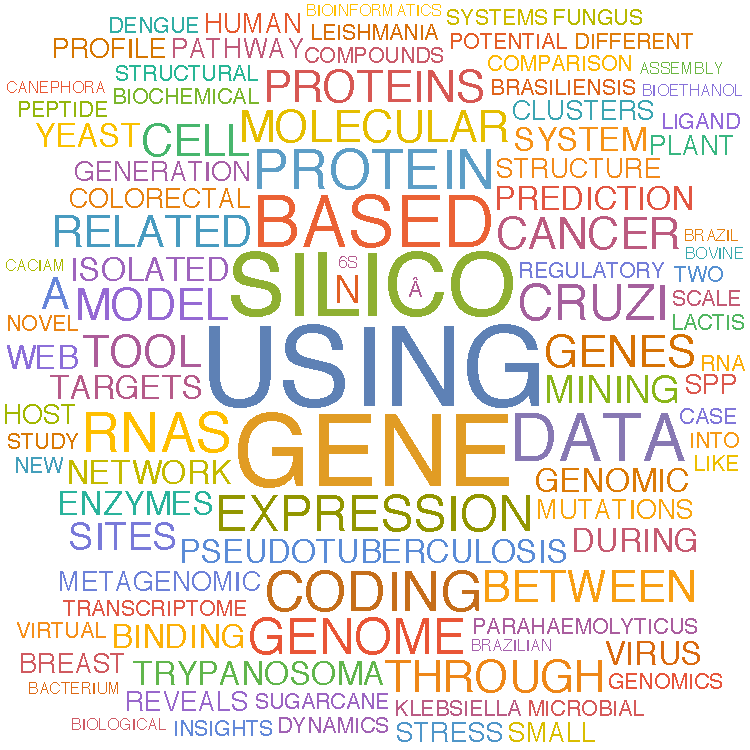
\includegraphics[scale=0.7]{wordcloud}
\end{center}
\caption{Word Cloud for the words used on the Conference Papers Titles}
\end{figure}
\chapter{Abstracts}
%\clearpage
%\includepdf{papers/artFP01.pdf}
%\clearpage
\procday{Poster Session}

\session{Genes and Genomics}

\procpaper[switch=45,
title={Design of chimeric antigens of Porcine Reproductive and Respiratory Syndrome Virus (PRRSV) through bioinformatics approaches: a rational model for the development of a diagnostic test}, 
     author={Jerusa Botelho Souza,Giuliana Loreto Saraiva, Jacksonde Andrade Teixeira, Pedro Marcus Pereira Vidigal, M�rcia Rog�riade Almeida Lam�go}, 
  index={\index{Souza, Jerusa Botelho}\index{Saraiva, Giuliana Loreto}\index{Teixeira, Jacksonde Andrade}\index{Vidigal, Pedro Marcus Pereira}\index{Lam�go, M�rcia Rog�riade Almeida}}]
{36229}

\procpaper[switch=45,
title={Prediction of microRNAs and miRNA pathway genes in Solanum lycopersicum and Solanum pennellii}, 
     author={Tha�s Cunhade Sousa Cardoso,Tamires Caixeta Alves, Carolina Milagres Caneschi, Douglas Santana, Laurence Rodrigues do Amaral, Luiz Ant�nio Augusto Gomes, Wilson Roberto Maluf, Matheusde Souza Gomes}, 
  index={\index{Cardoso, Tha�s Cunhade Sousa}\index{Alves, Tamires Caixeta}\index{Caneschi, Carolina Milagres}\index{Santana, Douglas}\index{Amaral, Laurence Rodrigues do}\index{Gomes, Luiz Ant�nio Augusto}\index{Maluf, Wilson Roberto}\index{Gomes, Matheusde Souza}}]
{36368}

\procpaper[switch=45,
title={In silico genomic analysis of the endophytic bacterium Bacillus amyloliquefaciens 629}, 
     author={Brena Mota Moitinho Sant'anna,Artur Trancoso Lopode Queiroz, Milton Ricardode Abreu Roque}, 
  index={\index{Sant'anna, Brena Mota Moitinho}\index{Queiroz, Artur Trancoso Lopode}\index{Roque, Milton Ricardode Abreu}}]
{36437}

\procpaper[switch=45,
title={Genotoxicity testing in-silico: quantification of the DNA mutation caused by the glycosidic bond hydrolysis}, 
     author={B�rbara Zanandreizde Siqueira Mattos,Gustavo Henrique Passini Santos, Anton Semenchenko}, 
  index={\index{Mattos, B�rbara Zanandreizde Siqueira}\index{Santos, Gustavo Henrique Passini}\index{Semenchenko, Anton}}]
{36641}

\procpaper[switch=45,
title={Admixture Mapping of Brazilians Identifies New Obesity Susceptibility Loci}, 
     author={Hanaisade Pla E Sant Anna,Marilia Scliar, Meddly L. Santolalla Robles, Thiago Peixoto Leal, Gilderlanio Santanade Ara�jo, Mateus Gouveia, Wagner Magalhaes, Fernanda Kehdy, Eduardo Martin Tarazona Santos}, 
  index={\index{Anna, Hanaisade Pla E Sant}\index{Scliar, Marilia}\index{Robles, Meddly L. Santolalla}\index{Leal, Thiago Peixoto}\index{Ara�jo, Gilderlanio Santanade}\index{Gouveia, Mateus}\index{Magalhaes, Wagner}\index{Kehdy, Fernanda}\index{Santos, Eduardo Martin Tarazona}}]
{36697}

\procpaper[switch=45,
title={Diagnostic metagenomics: a case study based on suspected dengue infection}, 
     author={Liliane Conteville,Michel Abanto Mar�n, Ana Maria Bispode Filippis, Rita Maria Ribeiro Nogueira, Marcos C�sar Limade Mendon�a, Ana Carolina Paulo Vicente}, 
  index={\index{Conteville, Liliane}\index{Mar�n, Michel Abanto}\index{Filippis, Ana Maria Bispode}\index{Nogueira, Rita Maria Ribeiro}\index{Mendon�a, Marcos C�sar Limade}\index{Vicente, Ana Carolina Paulo}}]
{36767}

\procpaper[switch=45,
title={Detection of Functional Analogous Enzymes in the Human Metabolism}, 
     author={Rafael Mina Piergiorge,Ana Carolina Ramos Guimar�es, Marcos Paulo Catanhode Souza}, 
  index={\index{Piergiorge, Rafael Mina}\index{Guimar�es, Ana Carolina Ramos}\index{Souza, Marcos Paulo Catanhode}}]
{36776}

\procpaper[switch=45,
title={tRNA array genomic survey unravels their presence and structure in Mycobacteria}, 
     author={Sergio Mascarenhas Morgado,Ana Carolina Paulo Vicente, Michel Abanto Mar�n}, 
  index={\index{Morgado, Sergio Mascarenhas}\index{Vicente, Ana Carolina Paulo}\index{Mar�n, Michel Abanto}}]
{36785}

\procpaper[switch=45,
title={The first complete genome sequence of Streptococcus dysgalatiae subsp. dysgalactiae an emerging fish pathogen}, 
     author={Alexandra Antonieta Urrutia Zegarra,Felipe Luiz Pereira, Fernanda Alves Dorella, Alex F. Carvalho, Gustavo Morais  Barony, Carlos A. G. Leal, Henrique Figueiredo}, 
  index={\index{Zegarra, Alexandra Antonieta Urrutia}\index{Pereira, Felipe Luiz}\index{Dorella, Fernanda Alves}\index{Carvalho, Alex F.}\index{Barony, Gustavo Morais }\index{Leal, Carlos A. G.}\index{Figueiredo, Henrique}}]
{36881}

\procpaper[switch=45,
title={Assembly, annotation and comparison of Corynebacterium pseudotuberculosis lineages}, 
     author={Doglas Parise,Thiagode Jesus Sousa, Mariana Teixeira Dornelles Parise, Adrian Valent�n Mu�oz Bucio, Felipe Luiz Pereira, Fernanda Alves Dorella, Efr�n D�az Aparicio, Henrique Figueiredo, Daniela Arruda Costa, Vasco Ade C Azevedo}, 
  index={\index{Parise, Doglas}\index{Sousa, Thiagode Jesus}\index{Parise, Mariana Teixeira Dornelles}\index{Bucio, Adrian Valent�n Mu�oz}\index{Pereira, Felipe Luiz}\index{Dorella, Fernanda Alves}\index{Aparicio, Efr�n D�az}\index{Figueiredo, Henrique}\index{Costa, Daniela Arruda}\index{Azevedo, Vasco Ade C}}]
{37027}

\procpaper[switch=45,
title={Identification of Specific Enzymes in the Comparison between Fusarium oxysporum and Arabidopsis thaliana}, 
     author={Larissa Catharina Costa,Nicolas Carels}, 
  index={\index{Costa, Larissa Catharina}\index{Carels, Nicolas}}]
{37064}

\procpaper[switch=45,
title={A comparative in silico linear B-cell epitope prediction for South American and African Trypanosoma vivax strains}, 
     author={Rafael Lucas Muniz Guedes,Carla Monadeli Filgueira Rodrigues, Luiz Gonzaga Paulade Almeida, Paola Minoprio, Marta Maria Geraldes Teixeira, Ana Tereza Ribeirode Vasconcelos}, 
  index={\index{Guedes, Rafael Lucas Muniz}\index{Rodrigues, Carla Monadeli Filgueira}\index{Almeida, Luiz Gonzaga Paulade}\index{Minoprio, Paola}\index{Teixeira, Marta Maria Geraldes}\index{Vasconcelos, Ana Tereza Ribeirode}}]
{37072}

\procpaper[switch=45,
title={Within and between gene variants: tracking for potential targets for populational linkage according to the metagenomic profile in a changing freshwater environment}, 
     author={Marcele Laux,Ricardo Assun��o Vialle, Jos� Miguel Ortega, Alessandra Giani}, 
  index={\index{Laux, Marcele}\index{Vialle, Ricardo Assun��o}\index{Ortega, Jos� Miguel}\index{Giani, Alessandra}}]
{37154}

\procpaper[switch=45,
title={Draft genome of Serratia marcescens UENF 22-GI: a plant growth promoting bacterium isolated from vermicompost}, 
     author={Filipe Pereira Matteoli,Pollyanna Santiago Lopes, F�bio Lopes Olivares, Thiago Motta Venancio}, 
  index={\index{Matteoli, Filipe Pereira}\index{Lopes, Pollyanna Santiago}\index{Olivares, F�bio Lopes}\index{Venancio, Thiago Motta}}]
{37245}

\procpaper[switch=45,
title={Variant in the PDE4B related to Acute Lymphoblastic Leukemia relapse is differentiated in Native Americans}, 
     author={Rennan Garcias Moreira,Fernanda Rodrigues Soares, Eduardo Martin Tarazona Santos}, 
  index={\index{Moreira, Rennan Garcias}\index{Soares, Fernanda Rodrigues}\index{Santos, Eduardo Martin Tarazona}}]
{37251}

\procpaper[switch=45,
title={LTR retrotransposons in Hemileia vastatrix genome}, 
     author={Rafaela Leite Prado Rocha,Pedro Ricardo Rossi Marques Barreirros, Tiago Ant�niode Oliveira Mendes, La�rcio Zambolim, Ney Sussumu Sakiyama, Eveline Teixeira Caixeta}, 
  index={\index{Rocha, Rafaela Leite Prado}\index{Barreirros, Pedro Ricardo Rossi Marques}\index{Mendes, Tiago Ant�niode Oliveira}\index{Zambolim, La�rcio}\index{Sakiyama, Ney Sussumu}\index{Caixeta, Eveline Teixeira}}]
{37266}

\procpaper[switch=45,
title={Linear Algebra Methods for Inferring Phylogenies Based on Peptides Frequencies Vectors: An Efficient Alternative Method to Investigate Relationships among Genes, Genomes and Organisms}, 
     author={Braulio Roberto Gon�alves Marinho Couto,Lara Maria Silva Miranda, Gabriel Bandeira Tofani, Gustavo Palmer Irffi, Lucas Felipe Silva, Matheus Allef Cruz, Thiago do Carmo Librelon Rocha, Marcos Augusto Dos Santos}, 
  index={\index{Couto, Braulio Roberto Gon�alves Marinho}\index{Miranda, Lara Maria Silva}\index{Tofani, Gabriel Bandeira}\index{Irffi, Gustavo Palmer}\index{Silva, Lucas Felipe}\index{Cruz, Matheus Allef}\index{Rocha, Thiago do Carmo Librelon}\index{Santos, Marcos Augusto Dos}}]
{37273}

\procpaper[switch=45,
title={The genomic basis for the variable biochemical profiles that lead to erroneous identifications of emerging pathogenic Corynebacterium spp.}, 
     author={Andr�de Souza Santos,Luis Gustavo Carvalho Pacheco, Carolina S. Silva, Catarina A. Moreira, Artur Silva, Vasco Ade C Azevedo, Liza F. Vilela}, 
  index={\index{Santos, Andr�de Souza}\index{Pacheco, Luis Gustavo Carvalho}\index{Silva, Carolina S.}\index{Moreira, Catarina A.}\index{Silva, Artur}\index{Azevedo, Vasco Ade C}\index{Vilela, Liza F.}}]
{37287}

\procpaper[switch=45,
title={Inferring the genetic structure and the history of interaction between Andean and Amazonian human populations using genome-wide data}, 
     author={Victor Octavio Borda Pua,Marilia Scliar, Mateus Gouveia, Thiago Peixoto Leal, Gilderlanio Santanade Ara�jo, Giordano Souza, Robert H Gilman, Heinner Guio, Eduardo Martin Tarazona Santos}, 
  index={\index{Pua, Victor Octavio Borda}\index{Scliar, Marilia}\index{Gouveia, Mateus}\index{Leal, Thiago Peixoto}\index{Ara�jo, Gilderlanio Santanade}\index{Souza, Giordano}\index{Gilman, Robert H}\index{Guio, Heinner}\index{Santos, Eduardo Martin Tarazona}}]
{37311}

\procpaper[switch=45,
title={Genotypic characterization of Vibrio parahaemolyticus strains isolated in Brazil}, 
     author={Crist�v�o Antunesde Lanna,Leandrode Oliveira Santos, Paulo Bisch, Wanda Von Kr�ger}, 
  index={\index{Lanna, Crist�v�o Antunesde}\index{Santos, Leandrode Oliveira}\index{Bisch, Paulo}\index{Kr�ger, Wanda Von}}]
{37312}

\procpaper[switch=45,
title={Searching for genomic elements of sexual reproduction in a microsporidian pathogen}, 
     author={Julianode Oliveira Silveira,Karen Luisa Haag, Jean-fran�ois Pombert}, 
  index={\index{Silveira, Julianode Oliveira}\index{Haag, Karen Luisa}\index{Pombert, Jean-fran�ois}}]
{37313}

\procpaper[switch=45,
title={Identification and variability analysis of monooxygenase gene family from Chrysoporthe cubensis}, 
     author={T�lio Morgan,Murillo Peterlini Tavares, Rafaela In�sde Souza Ladeira �zar, Tiago Ant�niode Oliveira Mendes, Val�ria Monteze Guimar�es}, 
  index={\index{Morgan, T�lio}\index{Tavares, Murillo Peterlini}\index{�zar, Rafaela In�sde Souza Ladeira}\index{Mendes, Tiago Ant�niode Oliveira}\index{Guimar�es, Val�ria Monteze}}]
{37346}

\procpaper[switch=45,
title={In silico prediction of auxiliary activity enzymes secreted by the fungus Chrysoporthe cubensis}, 
     author={Murillo Peterlini Tavares,T�lio Morgan, Thiago Rodrigues Dutra, Tiago Ant�niode Oliveira Mendes, Hugo Rody Vianna Silva, Val�ria Monteze Guimar�es}, 
  index={\index{Tavares, Murillo Peterlini}\index{Morgan, T�lio}\index{Dutra, Thiago Rodrigues}\index{Mendes, Tiago Ant�niode Oliveira}\index{Silva, Hugo Rody Vianna}\index{Guimar�es, Val�ria Monteze}}]
{37350}

\procpaper[switch=45,
title={A novel hierarchical in silico approach for the prediction of drug and vaccine targets against Chlamydophila pneumoniae}, 
     author={Ana Carolina Barbosa Caetano,}, 
  index={\index{Caetano, Ana Carolina Barbosa}}]
{37351}

\procpaper[switch=45,
title={Establishment of a pipeline for 16S-based metagenomic studies of Mycobacterium leprae}, 
     author={Felipe Borim Correa,Gabriel da Rocha Fernandes}, 
  index={\index{Correa, Felipe Borim}\index{Fernandes, Gabriel da Rocha}}]
{37381}

\procpaper[switch=45,
title={Impact of non-synonymous mutations in adaptive diversification and domestication of soybean}, 
     author={Kanhu Charan Moharana,Thiago Motta Venancio}, 
  index={\index{Moharana, Kanhu Charan}\index{Venancio, Thiago Motta}}]
{37449}

\procpaper[switch=45,
title={Prediction and analysis of plasmids from multidrug-resistant Klebsiella pneumoniae and Enterobacter aerogenes clinical isolates}, 
     author={Hemanoel Passarelli Araujo,Filipe Pereira Matteoli, Jussara Kasuko Palmeiro, L�bera Dalla-costa, Thiago Motta Venancio}, 
  index={\index{Araujo, Hemanoel Passarelli}\index{Matteoli, Filipe Pereira}\index{Palmeiro, Jussara Kasuko}\index{Dalla-costa, L�bera}\index{Venancio, Thiago Motta}}]
{37454}

\procpaper[switch=45,
title={Chromosomal copy number variation reveals extensive levels of genomic plasticity among and within Trypanosoma cruzi DTUs}, 
     author={Jo�o Lu�s Reis Cunha,Gabriela Flavia Rodrigues Luiz, Hugo O. Valdivia, Rodrigo P. Baptista, Laila Almeida, Mariana Santos Cardoso, Tiago Ant�niode Oliveira Mendes, Andrea M. Macedo, Ana Tereza Ribeirode Vasconcelos, Gustavo Coutinho Cerqueira, Daniella Bartholomeu}, 
  index={\index{Cunha, Jo�o Lu�s Reis}\index{Luiz, Gabriela Flavia Rodrigues}\index{Valdivia, Hugo O.}\index{Baptista, Rodrigo P.}\index{Almeida, Laila}\index{Cardoso, Mariana Santos}\index{Mendes, Tiago Ant�niode Oliveira}\index{Macedo, Andrea M.}\index{Vasconcelos, Ana Tereza Ribeirode}\index{Cerqueira, Gustavo Coutinho}\index{Bartholomeu, Daniella}}]
{37456}

\procpaper[switch=45,
title={Modular variability of multigene families encoding surface proteins uncovers differential composition of motifs among Trypanosoma cruzi strains}, 
     author={Jo�o Lu�s Reis Cunha,Gabriela Flavia Rodrigues Luiz, Rodrigo P. Baptista, Laila Almeida, Mariana Santos Cardoso, Gustavo Coutinho Cerqueira, Daniella Bartholomeu}, 
  index={\index{Cunha, Jo�o Lu�s Reis}\index{Luiz, Gabriela Flavia Rodrigues}\index{Baptista, Rodrigo P.}\index{Almeida, Laila}\index{Cardoso, Mariana Santos}\index{Cerqueira, Gustavo Coutinho}\index{Bartholomeu, Daniella}}]
{37461}

\procpaper[switch=45,
title={Genomic identification and patterns of expression of secondary metabolite gene clusters in the entomopathogen fungus Metarhizium anisopliae.}, 
     author={Augusto Schrank,Nicolau Sbaraini}, 
  index={\index{Schrank, Augusto}\index{Sbaraini, Nicolau}}]
{37470}

\procpaper[switch=45,
title={Genome analysis of E. nigrum and other filamentous fungi reveals molecular mechanisms related to endophytic/pathogenic lifestyles}, 
     author={Almir Jos� Ferreira,Liliane Santana Oliveira Kashiwabara, Jo�o M. P. Alves, Michael Thon, Alan M. Durham, L�ia C. L. F�varo, Arthur Gruber, Welington L. Ara�jo}, 
  index={\index{Ferreira, Almir Jos�}\index{Kashiwabara, Liliane Santana Oliveira}\index{Alves, Jo�o M. P.}\index{Thon, Michael}\index{Durham, Alan M.}\index{F�varo, L�ia C. L.}\index{Gruber, Arthur}\index{Ara�jo, Welington L.}}]
{37486}

\procpaper[switch=45,
title={Combining profile Hidden Markov Models and small RNA pattern based strategies to identify novel Endogenous Viral Elements (EVEs) and exogenous viruses}, 
     author={Arthur Gruber,Eric Roberto Guimar�es Rocha Aguiar, Liliane Santana Oliveira Kashiwabara, Jo�o M. P. Alves, Jo�o T. Marques}, 
  index={\index{Gruber, Arthur}\index{Aguiar, Eric Roberto Guimar�es Rocha}\index{Kashiwabara, Liliane Santana Oliveira}\index{Alves, Jo�o M. P.}\index{Marques, Jo�o T.}}]
{37512}

\procpaper[switch=45,
title={Preliminary analysis of functional SNPs mining from GBS data using GATK in a sugarcane map population}, 
     author={Alexandre Hild Aono,Estela Araujo Costa, Hugo Rody Vianna Silva, James Shiniti Nagai, Anete Pereirade Souza, Reginaldo Massanobu Kuroshu}, 
  index={\index{Aono, Alexandre Hild}\index{Costa, Estela Araujo}\index{Silva, Hugo Rody Vianna}\index{Nagai, James Shiniti}\index{Souza, Anete Pereirade}\index{Kuroshu, Reginaldo Massanobu}}]
{37556}

\procpaper[switch=45,
title={GBS data from a population of modern sugarcane variety reveals duplicate genes retained by breeding process}, 
     author={James Shiniti Nagai,Hugo Rody Vianna Silva, Estela Araujo Costa, Alexandre Hild Aono, Anete Pereirade Souza, Reginaldo Massanobu Kuroshu}, 
  index={\index{Nagai, James Shiniti}\index{Silva, Hugo Rody Vianna}\index{Costa, Estela Araujo}\index{Aono, Alexandre Hild}\index{Souza, Anete Pereirade}\index{Kuroshu, Reginaldo Massanobu}}]
{37575}

\procpaper[switch=45,
title={Characterization of phage sequences on Corynebacterium pseudotuberculosis genomes}, 
     author={Flavia Figueira Aburjaile,Am�lia Raiana F. Lobato, Lu�s Carlos Guimar�es, Ana L�dia Queiroz Cavalcante, Kenny da Costa Pinheiro, Adonney Allande Oliveira Veras, Rafael Azevedo Bara�na, Artur Silva, Rommel Thiago Juc� Ramos}, 
  index={\index{Aburjaile, Flavia Figueira}\index{Lobato, Am�lia Raiana F.}\index{Guimar�es, Lu�s Carlos}\index{Cavalcante, Ana L�dia Queiroz}\index{Pinheiro, Kenny da Costa}\index{Veras, Adonney Allande Oliveira}\index{Bara�na, Rafael Azevedo}\index{Silva, Artur}\index{Ramos, Rommel Thiago Juc�}}]
{37799}

\procpaper[switch=45,
title={Comparative genomic analysis of clinical and environmental strains of Vibrio parahaemolyticus isolated in Brazil: insight into their virulence potencial}, 
     author={Leandrode Oliveira Santos,Paulo Bisch, Wanda Von Kr�ger}, 
  index={\index{Santos, Leandrode Oliveira}\index{Bisch, Paulo}\index{Kr�ger, Wanda Von}}]
{37921}

\procpaper[switch=45,
title={Identification of Pho regulon genes and Pho box-like sequences in genomes of clinical and environmental isolates of Vibrio parahaemolyticus from Brazil}, 
     author={Leandrode Oliveira Santos,Crist�v�o Antunesde Lanna, Paulo Bisch, Wanda Von Kr�ger}, 
  index={\index{Santos, Leandrode Oliveira}\index{Lanna, Crist�v�o Antunesde}\index{Bisch, Paulo}\index{Kr�ger, Wanda Von}}]
{37922}

\procpaper[switch=45,
title={Identification of genetic variations in engineered yeast for xylose consumption and acetic acid resistance applied to second generation ethanol production}, 
     author={Sheila Tiemi Nagamatsu,Luige Armando Llerena Calderon, Lucas Parreiras, Bruna Tatsue, Angelica Martins Gomes, Gon�alo Amarante Guimar�es Pereira, Marcelo Falsarella Carazzolle}, 
  index={\index{Nagamatsu, Sheila Tiemi}\index{Calderon, Luige Armando Llerena}\index{Parreiras, Lucas}\index{Tatsue, Bruna}\index{Gomes, Angelica Martins}\index{Pereira, Gon�alo Amarante Guimar�es}\index{Carazzolle, Marcelo Falsarella}}]
{37972}

\procpaper[switch=45,
title={In silico approaches to predict the impact of leukemic DNMT3a mutations \& Identification of leads based on drug decitabine using Complex Based Pharmacophore Mapping and Virtual Screening}, 
     author={Syed Babar Jamal Bacha,Matheus Filgueira Bezerra, Sandeep Tiwari, Flavia Figueira Aburjaile, Vasco Ade C Azevedo, Artur Silva, Cintia Renata Rocha Costa, Marcos Andr� Calvancanti Bezerra, Antonio Roberto Lucena-araujo, Eduardo Isidoro Carneiro Beltr�o}, 
  index={\index{Bacha, Syed Babar Jamal}\index{Bezerra, Matheus Filgueira}\index{Tiwari, Sandeep}\index{Aburjaile, Flavia Figueira}\index{Azevedo, Vasco Ade C}\index{Silva, Artur}\index{Costa, Cintia Renata Rocha}\index{Bezerra, Marcos Andr� Calvancanti}\index{Lucena-araujo, Antonio Roberto}\index{Beltr�o, Eduardo Isidoro Carneiro}}]
{38218}

\procpaper[switch=45,
title={In-silico analyses for the discovery of drug and vaccine targets in Corynebacterium camporealensis: A Novel Hierarchical Approach}, 
     author={Syed Babar Jamal Bacha,Sandeep Tiwari, Arun Kumar Jaiswal, Daniela Arruda Costa, Doglas Parise, Henrique Cp Figueiredo, Debmalya Barh, Artur Silva, Vasco Ade C Azevedo}, 
  index={\index{Bacha, Syed Babar Jamal}\index{Tiwari, Sandeep}\index{Jaiswal, Arun Kumar}\index{Costa, Daniela Arruda}\index{Parise, Doglas}\index{Figueiredo, Henrique Cp}\index{Barh, Debmalya}\index{Silva, Artur}\index{Azevedo, Vasco Ade C}}]
{38219}

\procpaper[switch=45,
title={Genotype imputation of Hereford and Bradford bovine breeds from Brazil}, 
     author={Mauriciode Alvarenga Mudadu,Henry Gomesde Carvalho, Marcos Jun Iti Yokoo, Fernando Flores Cardoso}, 
  index={\index{Mudadu, Mauriciode Alvarenga}\index{Carvalho, Henry Gomesde}\index{Yokoo, Marcos Jun Iti}\index{Cardoso, Fernando Flores}}]
{38309}

\procpaper[switch=45,
title={Detection of potential genetic variants affecting gene function in Guzerat cattle}, 
     author={Adhemar Zerlotini Neto,}, 
  index={\index{Neto, Adhemar Zerlotini}}]
{38352}

\procpaper[switch=45,
title={Characterization of the probiotic and stress resistance-related genes of Lactococcus lactis subsp. lactis NCDO 2118 through comparative genomics and in vitro assays.}, 
     author={Let�ciade Castro Oliveira,}, 
  index={\index{Oliveira, Let�ciade Castro}}]
{38402}

\procpaper[switch=45,
title={A comparison of two pipelines for metagenomic 16S rRNA using Ion Torrent (PGM) Sequencing Platform}, 
     author={Daniel Vasconcelos Rissi,Suzana Eiko Sato Guima, Rodrigo Matheus Pereira}, 
  index={\index{Rissi, Daniel Vasconcelos}\index{Guima, Suzana Eiko Sato}\index{Pereira, Rodrigo Matheus}}]
{38438}

\procpaper[switch=45,
title={Insights into Klebsiella penumoniae type VI secretion system regulation}, 
     author={Victor Barbosa,Leticia Ms Lery}, 
  index={\index{Barbosa, Victor}\index{Lery, Leticia Ms}}]
{38477}

\procpaper[switch=45,
title={AMP-Identifier: A Unix shell script for antimicrobial peptide identification}, 
     author={Jo�o Pacifico Bezerra Neto,Mauro Guida Dos Santos, Ana Maria Benko-iseppon}, 
  index={\index{Neto, Jo�o Pacifico Bezerra}\index{Santos, Mauro Guida Dos}\index{Benko-iseppon, Ana Maria}}]
{38488}

\procpaper[switch=45,
title={Genome mining of biosynthetic gene clusters in Nostoc sp. CACIAM 19, a cyanobacterium from an Amazonian environment}, 
     author={David Batista Mau�s,Alex Ranieri Jer�nimo Lima, Pablo Henrique Gon�alves Moraes, Andrei Santos Siqueira, Leonardo Teixeira Dall'agnol, Evonnildo Costa Gon�alves}, 
  index={\index{Mau�s, David Batista}\index{Lima, Alex Ranieri Jer�nimo}\index{Moraes, Pablo Henrique Gon�alves}\index{Siqueira, Andrei Santos}\index{Dall'agnol, Leonardo Teixeira}\index{Gon�alves, Evonnildo Costa}}]
{38511}

\procpaper[switch=45,
title={Ab initio characterization of promoter regions based on Conditional Random Fields}, 
     author={�gor Bonadio,Maurode Medeiros Oliveira, Alan Durham}, 
  index={\index{Bonadio, �gor}\index{Oliveira, Maurode Medeiros}\index{Durham, Alan}}]
{38513}

\procpaper[switch=45,
title={Study of Chromatin Remodeling in Colorectal Cancer Progression}, 
     author={Simone Nantesde Aquino,Nicole Scherer, Mariana Boroni}, 
  index={\index{Aquino, Simone Nantesde}\index{Scherer, Nicole}\index{Boroni, Mariana}}]
{38525}

\procpaper[switch=45,
title={Taxonomic identification of metagenomics reads based on sequence features by Support Vector Machines (SVM)}, 
     author={Tahila Andrighetti,Ney Lemke}, 
  index={\index{Andrighetti, Tahila}\index{Lemke, Ney}}]
{38526}

\procpaper[switch=45,
title={Cell cycle and metabolism related candidate human synthetic lethal network}, 
     author={Sandeep Tiwari,Thiago Luizde Paula Castro, N�bia Seiffert, Debmalya Barh, Vasco Ade C Azevedo}, 
  index={\index{Tiwari, Sandeep}\index{Castro, Thiago Luizde Paula}\index{Seiffert, N�bia}\index{Barh, Debmalya}\index{Azevedo, Vasco Ade C}}]
{38528}

\procpaper[switch=45,
title={The discovery of novel multiple small deletions within human coding genes associated to known lung cancer pathways.}, 
     author={Gabriel Wajnberg,Raphael Tavares da Silva, Nicole Scherer, Carlos Gil Ferreira, Fabio Passetti}, 
  index={\index{Wajnberg, Gabriel}\index{Silva, Raphael Tavares da}\index{Scherer, Nicole}\index{Ferreira, Carlos Gil}\index{Passetti, Fabio}}]
{38531}

\procpaper[switch=45,
title={Identification of somatic mutations in prostate adenocarcinoma with Gleason score 7 and 8 and their associations with biochemical recurrence}, 
     author={Isabella Tanus Job E Meira,Bruna D F Barros, Rodrigo F Ramalho, Jos� E Kroll, Renan Valieres, Sandro Josede Souza, Isabela W da Cunha, Gustavo C Guimar�es, Dirce M Carraro, Elisa N Ferreira}, 
  index={\index{Meira, Isabella Tanus Job E}\index{Barros, Bruna D F}\index{Ramalho, Rodrigo F}\index{Kroll, Jos� E}\index{Valieres, Renan}\index{Souza, Sandro Josede}\index{Cunha, Isabela W da}\index{Guimar�es, Gustavo C}\index{Carraro, Dirce M}\index{Ferreira, Elisa N}}]
{38573}

\procpaper[switch=45,
title={Detection and correction mis-assemblies in genome of Corynebacterium pseudotuberculosis}, 
     author={Thiagode Jesus Sousa,Doglas Parise, Diego C�sar Batista Mariano, Daniela Arruda Costa, Felipe Luiz Pereira, Henrique Figueiredo, Artur Silva, Rommel Thiago Juc� Ramos, Vasco Ade C Azevedo}, 
  index={\index{Sousa, Thiagode Jesus}\index{Parise, Doglas}\index{Mariano, Diego C�sar Batista}\index{Costa, Daniela Arruda}\index{Pereira, Felipe Luiz}\index{Figueiredo, Henrique}\index{Silva, Artur}\index{Ramos, Rommel Thiago Juc�}\index{Azevedo, Vasco Ade C}}]
{38686}

\procpaper[switch=45,
title={Genomic analysis of opportunistic bacteria from Herbaspirillum genus isolated from immunocompromised patients}, 
     author={Helisson Faoro,Willian Klassende Oliveira, Michelle Zibetti Tadra-sfeir, Rodrigo Luis Cardoso, Emanuel Maltempide Souza, Fabiode Oliveira Pedrosa}, 
  index={\index{Faoro, Helisson}\index{Oliveira, Willian Klassende}\index{Tadra-sfeir, Michelle Zibetti}\index{Cardoso, Rodrigo Luis}\index{Souza, Emanuel Maltempide}\index{Pedrosa, Fabiode Oliveira}}]
{38704}

\procpaper[switch=45,
title={Investigation of mutations in the HBB gene using the 1000 GENOMES databank}, 
     author={Tania Carlice Lopes Pereira Dos Reis,Jaime Viana, Fabiano Moreira Cordeiro, Greicede Lemos Cardoso, Jo�o Guerreiro, Sidney Santos, �ndrea Kely Campos Ribeiro Dos Santos}, 
  index={\index{Reis, Tania Carlice Lopes Pereira Dos}\index{Viana, Jaime}\index{Cordeiro, Fabiano Moreira}\index{Cardoso, Greicede Lemos}\index{Guerreiro, Jo�o}\index{Santos, Sidney}\index{Santos, �ndrea Kely Campos Ribeiro Dos}}]
{38718}

\procpaper[switch=45,
title={An hierarchical classification system for beta-lactamases}, 
     author={Melise Chaves Silveira,F�bio Mota, Rodrigo Jardim, Rangeline Azevedo da Silva, Marcos Paulo Catanhode Souza, Ana Carolina Ramos Guimar�es, Antonio Basiliode Miranda}, 
  index={\index{Silveira, Melise Chaves}\index{Mota, F�bio}\index{Jardim, Rodrigo}\index{Silva, Rangeline Azevedo da}\index{Souza, Marcos Paulo Catanhode}\index{Guimar�es, Ana Carolina Ramos}\index{Miranda, Antonio Basiliode}}]
{38729}

\procpaper[switch=45,
title={Draft genome sequence of the extremophile endemic marine antarctic yeast Metchnikowia australis}, 
     author={Heron Hil�rio,Thiago Mafra Batista, Rennan Garcias Moreira, Val�ria Martins Godinho, Carlos Augusto Rosa, Luiz Henrique Rosa, Gl�ria Regina Franco}, 
  index={\index{Hil�rio, Heron}\index{Batista, Thiago Mafra}\index{Moreira, Rennan Garcias}\index{Godinho, Val�ria Martins}\index{Rosa, Carlos Augusto}\index{Rosa, Luiz Henrique}\index{Franco, Gl�ria Regina}}]
{38746}

\procpaper[switch=45,
title={Diversity analysis of Howler monkey (Alouatta spp.) fecal microbiota}, 
     author={Raquel Riyuzode Almeida Franco,Layla Martins, Jo�o Batista, Andrew Thomaz, Julio Oliveira, Aline Maria da Silva, Joao Carlos Setubal}, 
  index={\index{Franco, Raquel Riyuzode Almeida}\index{Martins, Layla}\index{Batista, Jo�o}\index{Thomaz, Andrew}\index{Oliveira, Julio}\index{Silva, Aline Maria da}\index{Setubal, Joao Carlos}}]
{38795}

\procpaper[switch=45,
title={Spacial Organization of Genomes: Insights on coordinated regulation of Biological Pathways}, 
     author={Lu�s Henrique,Jos� Miguel Ortega}, 
  index={\index{Henrique, Lu�s}\index{Ortega, Jos� Miguel}}]
{38799}

\procpaper[switch=45,
title={HD-zip classification in Vigna unguiculata and comparative synteny with Phaseolus vulgaris}, 
     author={Bruna Piereck Moura,Artemisa Nazar� Costa Borges, Carollinede Jes�s Pires, Fl�via Tadeude Ara�jo, Jos� Ribamar Costa Ferreira-neto, Ana Christina Brasileiro-vidal, Ana Maria Benko-iseppon}, 
  index={\index{Moura, Bruna Piereck}\index{Borges, Artemisa Nazar� Costa}\index{Pires, Carollinede Jes�s}\index{Ara�jo, Fl�via Tadeude}\index{Ferreira-neto, Jos� Ribamar Costa}\index{Brasileiro-vidal, Ana Christina}\index{Benko-iseppon, Ana Maria}}]
{38823}

\procpaper[switch=45,
title={CattleQTLdb analysis to increase understanding of the functions of milk proteins genes}, 
     author={Carolina Guimar�es Ramos Matosinho,Izinara Rosse da Cruz, Pablo Augustode Souza Fonseca, Juliana Assis, Francislon Silvade Oliveira, Fl�vio Marcos Gomes Ara�jo, Anna Christinade Matos Salim, Wagner Arbex, Marco Ant�nio Machado, Maria Gabriela Campolina Diniz Peixoto, Rui da Silva Verneque, Marta Fonseca Martins, Roney Santos Coimbra, Marcos Vin�cius Gualberto Barbosa da Silva, Guilherme Oliveira, Maria Raquel Santos Carvalho}, 
  index={\index{Matosinho, Carolina Guimar�es Ramos}\index{Cruz, Izinara Rosse da}\index{Fonseca, Pablo Augustode Souza}\index{Assis, Juliana}\index{Oliveira, Francislon Silvade}\index{Ara�jo, Fl�vio Marcos Gomes}\index{Salim, Anna Christinade Matos}\index{Arbex, Wagner}\index{Machado, Marco Ant�nio}\index{Peixoto, Maria Gabriela Campolina Diniz}\index{Verneque, Rui da Silva}\index{Martins, Marta Fonseca}\index{Coimbra, Roney Santos}\index{Silva, Marcos Vin�cius Gualberto Barbosa da}\index{Oliveira, Guilherme}\index{Carvalho, Maria Raquel Santos}}]
{38837}

\procpaper[switch=45,
title={In silico identification of the effects of genetic variants in transcription factors recognition sites in regulatory regions of candidate genes for reproductive disorders in cattle}, 
     author={Luizade Almeida Ferreira Diniz,Pablo Augustode Souza Fonseca, Ana Em�liade Paiva, Fernanda Caroline Santos, Izinara Rosse da Cruz, Maria Raquel Santos Carvalho}, 
  index={\index{Diniz, Luizade Almeida Ferreira}\index{Fonseca, Pablo Augustode Souza}\index{Paiva, Ana Em�liade}\index{Santos, Fernanda Caroline}\index{Cruz, Izinara Rosse da}\index{Carvalho, Maria Raquel Santos}}]
{38850}

\procpaper[switch=45,
title={Metagenomic analysis of the Southern Brazilian Atlantic Forest soil using next-generation sequencing technologies}, 
     author={Janynne Stephaniede Oliveira Palheta,Michelle Zibetti Tadra-sfeir, Emanuel Maltempide Souza, Fabiode Oliveira Pedrosa, Helisson Faoro}, 
  index={\index{Palheta, Janynne Stephaniede Oliveira}\index{Tadra-sfeir, Michelle Zibetti}\index{Souza, Emanuel Maltempide}\index{Pedrosa, Fabiode Oliveira}\index{Faoro, Helisson}}]
{38868}

\procpaper[switch=45,
title={Inference of distant homologs in Protozoa by pHMM–pHMM (profile Hidden Markov Model) comparison for the identification of superfamilies}, 
     author={Darueck Ac�cio Campos,Alberto M. R. D�vila, Rodrigo Jardim}, 
  index={\index{Campos, Darueck Ac�cio}\index{D�vila, Alberto M. R.}\index{Jardim, Rodrigo}}]
{38893}

\procpaper[switch=45,
title={Comparative Genomics between two different biovars of Corynebacterium pseudotuberculosis isolated in the same host}, 
     author={Rafael Cabus Gantois,Thiagode Jesus Sousa, Doglas Parise, Daniela Arruda Costa, Anne Cybelle Pinto Gomide, Henrique Figueiredo, Vasco Ade C Azevedo}, 
  index={\index{Gantois, Rafael Cabus}\index{Sousa, Thiagode Jesus}\index{Parise, Doglas}\index{Costa, Daniela Arruda}\index{Gomide, Anne Cybelle Pinto}\index{Figueiredo, Henrique}\index{Azevedo, Vasco Ade C}}]
{38906}

\procpaper[switch=45,
title={Relative Evaluation of NoSQL Databases For Manipulating Genotype Data}, 
     author={Arthur Lorenzi Almeida,Vinicius Schettino, Fernanda Nascimento Almeida, Wagner Arbex}, 
  index={\index{Almeida, Arthur Lorenzi}\index{Schettino, Vinicius}\index{Almeida, Fernanda Nascimento}\index{Arbex, Wagner}}]
{38936}

\procpaper[switch=45,
title={Metagenomics insights reveals functional patterns among soil microbial communities of global biomes}, 
     author={Melline Fontes Noronha,Gileno Vieira Lacerda Junior, Jack A Gilbert, Val�ria Maiade Oliveira}, 
  index={\index{Noronha, Melline Fontes}\index{Junior, Gileno Vieira Lacerda}\index{Gilbert, Jack A}\index{Oliveira, Val�ria Maiade}}]
{39144}

\procpaper[switch=45,
title={Complete genome sequence of Corynebacterium pseudotuberculosis 33}, 
     author={Marcus Vinicius Can�rio Viana,Doglas Parise, Thiagode Jesus Sousa, Leandrode Jesus Benevides, Diego C�sar Batista Mariano, Fl�viade Souza Rocha, Priscilla Bagano, Lu�s Carlos Guimar�es, Felipe Luiz Pereira, Fernanda Alves Dorella, Rommel Ramos, Salah Abdel Karim Selim, Mohammad Salaheldean, Artur Silva, Alice Rebecca Wattam, Vasco Ade C Azevedo}, 
  index={\index{Viana, Marcus Vinicius Can�rio}\index{Parise, Doglas}\index{Sousa, Thiagode Jesus}\index{Benevides, Leandrode Jesus}\index{Mariano, Diego C�sar Batista}\index{Rocha, Fl�viade Souza}\index{Bagano, Priscilla}\index{Guimar�es, Lu�s Carlos}\index{Pereira, Felipe Luiz}\index{Dorella, Fernanda Alves}\index{Ramos, Rommel}\index{Selim, Salah Abdel Karim}\index{Salaheldean, Mohammad}\index{Silva, Artur}\index{Wattam, Alice Rebecca}\index{Azevedo, Vasco Ade C}}]
{40196}

\session{Phylogeny and Evolution}

\procpaper[switch=45,
title={Evolution of heterotrophy: Genes needed for regulation of the acidity of pancreatic juice appeared recently in man evolution}, 
     author={Fen�cia Brito,Carlos Alberto Xavier Gon�alves, Jos� Miguel Ortega}, 
  index={\index{Brito, Fen�cia}\index{Gon�alves, Carlos Alberto Xavier}\index{Ortega, Jos� Miguel}}]
{36692}

\procpaper[switch=45,
title={Walking through old routes to reach new destinations: unraveling the origin of the mammary gland}, 
     author={Lissur Azevedo Orsine,Elisa Renn� Donnard Moreira, Jos� Miguel Ortega}, 
  index={\index{Orsine, Lissur Azevedo}\index{Moreira, Elisa Renn� Donnard}\index{Ortega, Jos� Miguel}}]
{36820}

\procpaper[switch=45,
title={Mosquitoes Mobilome}, 
     author={Gabriel da Luz Wallau,Elverson Soaresde Melo}, 
  index={\index{Wallau, Gabriel da Luz}\index{Melo, Elverson Soaresde}}]
{36971}

\procpaper[switch=45,
title={B-cell epitopes prediction in trypanosomatids genome core}, 
     author={Anderson Coqueiro Dos Santos,Leandro Martinsde Freitas}, 
  index={\index{Santos, Anderson Coqueiro Dos}\index{Freitas, Leandro Martinsde}}]
{37157}

\procpaper[switch=45,
title={Construction of alternative algorithm for development of phylogenetic trees using InterPro entries and frequency vectors of tri-peptide}, 
     author={Braulio Roberto Gon�alves Marinho Couto,Lucas Felipe Silva, Dalila Dominique Duarte Rocha, Lara Maria Silva Miranda, Matheus Allef Cruz, Thiago do Carmo Librelon Rocha, Marcos Augusto Dos Santos}, 
  index={\index{Couto, Braulio Roberto Gon�alves Marinho}\index{Silva, Lucas Felipe}\index{Rocha, Dalila Dominique Duarte}\index{Miranda, Lara Maria Silva}\index{Cruz, Matheus Allef}\index{Rocha, Thiago do Carmo Librelon}\index{Santos, Marcos Augusto Dos}}]
{37275}

\procpaper[switch=45,
title={Biological modules associated with prophage density in pathogenic and commensal Escherichia coli}, 
     author={Tarcisio Jos� Domingos Coutinho,Francisco Pereira Lobo, Gl�ria Regina Franco}, 
  index={\index{Coutinho, Tarcisio Jos� Domingos}\index{Lobo, Francisco Pereira}\index{Franco, Gl�ria Regina}}]
{37372}

\procpaper[switch=45,
title={Inferring the demographic history of Cnesterodon brevirostratus using bioinformatics tools}, 
     author={Daniela Ambros Quinsani,Martiela Vazde Freitas, Aline M.c. Ramos-fregonezi, Luis Roberto Malabarba, Nelson J.r. Fagundes}, 
  index={\index{Quinsani, Daniela Ambros}\index{Freitas, Martiela Vazde}\index{Ramos-fregonezi, Aline M.c.}\index{Malabarba, Luis Roberto}\index{Fagundes, Nelson J.r.}}]
{37406}

\procpaper[switch=45,
title={Improving the supertree approach by analyzing protein clusters with paralogs and including distance data}, 
     author={Tetsu Sakamoto,Jos� Miguel Ortega}, 
  index={\index{Sakamoto, Tetsu}\index{Ortega, Jos� Miguel}}]
{37439}

\procpaper[switch=45,
title={Reconstructing ancestral protein-protein interactions of virus-host systems}, 
     author={Anderson Fernandesde Brito,John W. Pinney}, 
  index={\index{Brito, Anderson Fernandesde}\index{Pinney, John W.}}]
{37543}

\procpaper[switch=45,
title={Study of the origin of the genes controlling flower development}, 
     author={Beatriz Moura Kfouryde Castro,Lab Biodados, Carlos Alberto Xavier Gon�alves}, 
  index={\index{Castro, Beatriz Moura Kfouryde}\index{Biodados, Lab}\index{Gon�alves, Carlos Alberto Xavier}}]
{37593}

\procpaper[switch=45,
title={Secondary structure changes according to evolutionary age}, 
     author={Ricardo Assun��o Vialle,Jos� Miguel Ortega}, 
  index={\index{Vialle, Ricardo Assun��o}\index{Ortega, Jos� Miguel}}]
{38369}

\procpaper[switch=45,
title={ProteinWorldDB in a multidimensional representation of the Network of Life}, 
     author={Edson Machado Filho,}, 
  index={\index{Filho, Edson Machado}}]
{38407}

\procpaper[switch=45,
title={GO-Genesis: finding the origin of biological processes and molecular functions from Gene Ontology}, 
     author={Carlos Alberto Xavier Gon�alves,Lab Biodados}, 
  index={\index{Gon�alves, Carlos Alberto Xavier}\index{Biodados, Lab}}]
{38520}

\procpaper[switch=45,
title={mtDNA Data Mining: A Global Analysis}, 
     author={Camilla Reginattode Pierri,Bruno Thiagode Lima Nichio, Tetsu Sakamoto, Mauro Ant�nio Alves Castro, Jos� Miguel Ortega, Roberto Tadeu Raittz}, 
  index={\index{Pierri, Camilla Reginattode}\index{Nichio, Bruno Thiagode Lima}\index{Sakamoto, Tetsu}\index{Castro, Mauro Ant�nio Alves}\index{Ortega, Jos� Miguel}\index{Raittz, Roberto Tadeu}}]
{38542}

\procpaper[switch=45,
title={Tardigrades (Ecdysozoa: Tardigrada) A general review of the record in gene database of Cytochrome Oxydase I (COI) and the Damage Suppressor gene (DSUP).}, 
     author={Antonio A A Pires,}, 
  index={\index{Pires, Antonio A A}}]
{38609}

\procpaper[switch=45,
title={Highly resolved phylogeny for Corynebacteriales}, 
     author={Nilson da Rocha Coimbra,Vasco Ade C Azevedo, A�da Ouangraoua}, 
  index={\index{Coimbra, Nilson da Rocha}\index{Azevedo, Vasco Ade C}\index{Ouangraoua, A�da}}]
{38613}

\procpaper[switch=45,
title={key amino acids in understanding evolutionary characterization of Mn/Fe-Superoxide Dismutase: A phylogenetic and structural analysis of proteins from Corynebacterium and hosts}, 
     author={Alberto F.de Oliveira Junior,Pammella Teixeira, Debmalya Barh, Preetam Ghosh, Vasco Ade C Azevedo}, 
  index={\index{Junior, Alberto F.de Oliveira}\index{Teixeira, Pammella}\index{Barh, Debmalya}\index{Ghosh, Preetam}\index{Azevedo, Vasco Ade C}}]
{38669}

\procpaper[switch=45,
title={Analysis of comparative genomics reveal evidence of positive selection on pathogenicity­-related genes of Witches' broom disease on cocoa trees}, 
     author={Paulo Massanari Tokimatu Filho,Juliana Jos�, Daniela Toledo Thomazella, Leandro Costa do Nascimento, Paulo Teixeira, Gon�alo Amarante Guimar�es Pereira, Marcelo Falsarella Carazzolle}, 
  index={\index{Filho, Paulo Massanari Tokimatu}\index{Jos�, Juliana}\index{Thomazella, Daniela Toledo}\index{Nascimento, Leandro Costa do}\index{Teixeira, Paulo}\index{Pereira, Gon�alo Amarante Guimar�es}\index{Carazzolle, Marcelo Falsarella}}]
{38690}

\procpaper[switch=45,
title={Analyzing molecular characteristics of small RNAs to assess the evolution of RNAi pathways}, 
     author={Eric Roberto Guimar�es Rocha Aguiar,Flavia Viana Ferreira, Roenick Proveti Olmo, Karla Pollyanna Vieirade Oliveira, Simona Paro, Isaque Jo�o da Silvade Faria, Bet�nia Paiva Drumond, Vinicius Augusto Carvalhode Abreu, Carine Meignin, Maur�cio Roberto Viana Sant'anna, Nelderde Figueiredo Gontijo, Luciano Andrade Moreira, Erna Geessien Kroon, Jean-luc Imler, Jo�o T. Marques}, 
  index={\index{Aguiar, Eric Roberto Guimar�es Rocha}\index{Ferreira, Flavia Viana}\index{Olmo, Roenick Proveti}\index{Oliveira, Karla Pollyanna Vieirade}\index{Paro, Simona}\index{Faria, Isaque Jo�o da Silvade}\index{Drumond, Bet�nia Paiva}\index{Abreu, Vinicius Augusto Carvalhode}\index{Meignin, Carine}\index{Sant'anna, Maur�cio Roberto Viana}\index{Gontijo, Nelderde Figueiredo}\index{Moreira, Luciano Andrade}\index{Kroon, Erna Geessien}\index{Imler, Jean-luc}\index{Marques, Jo�o T.}}]
{38720}

\procpaper[switch=45,
title={Evaluation of the accuracy of the MLrelate kinship analysis program when no parents are sampled}, 
     author={Leticia Ferreira Lima,Renata Schama}, 
  index={\index{Lima, Leticia Ferreira}\index{Schama, Renata}}]
{38731}

\procpaper[switch=45,
title={Assortative Mating in Brazilian Populations}, 
     author={Isabela Alvim,Hanaisade Pla E Sant Anna, Eduardo Martin Tarazona Santos}, 
  index={\index{Alvim, Isabela}\index{Anna, Hanaisade Pla E Sant}\index{Santos, Eduardo Martin Tarazona}}]
{38831}

\procpaper[switch=45,
title={Insights into the population history of free-living bacteria as counted by their CRISPR inventory}, 
     author={Julliane Dutra Medeiros,Laura Rabelo Leite, Francislon Silvade Oliveira, Victor Satler Pylro, Gabriel da Rocha Fernandes, Guilherme Oliveira, Sara Cuadros Orellana}, 
  index={\index{Medeiros, Julliane Dutra}\index{Leite, Laura Rabelo}\index{Oliveira, Francislon Silvade}\index{Pylro, Victor Satler}\index{Fernandes, Gabriel da Rocha}\index{Oliveira, Guilherme}\index{Orellana, Sara Cuadros}}]
{38854}

\procpaper[switch=45,
title={Evolutionary origin of the proteins involved in the entry of and defense to the Ebola virus in the host cell}, 
     author={Elisson Nogueira Lopes,Tetsu Sakamoto, Jos� Miguel Ortega}, 
  index={\index{Lopes, Elisson Nogueira}\index{Sakamoto, Tetsu}\index{Ortega, Jos� Miguel}}]
{38886}

\procpaper[switch=45,
title={Study of new molecular markers for Phylogenetic reconstruction of the black fungus in humans}, 
     author={Edgar Lacerdade Aguiar,Cl�udia Barbosa Assun��o, Rachel Basques Caligiorne}, 
  index={\index{Aguiar, Edgar Lacerdade}\index{Assun��o, Cl�udia Barbosa}\index{Caligiorne, Rachel Basques}}]
{38944}

\session{Proteins and Proteomics}

\procpaper[switch=45,
title={Molecular docking and structural optimization of bioactive compounds from natural products against 1-UAP of L. braziliensis}, 
     author={Sabrina Silva Mendon�a,Jo�o Marcos Gal�cio, Kelly Christina Ferreira Castro, Kau� Santana da Costa}, 
  index={\index{Mendon�a, Sabrina Silva}\index{Gal�cio, Jo�o Marcos}\index{Castro, Kelly Christina Ferreira}\index{Costa, Kau� Santana da}}]
{36197}

\procpaper[switch=45,
title={Cluster analysis of AcrB protein molecular dynamics conformations}, 
     author={N�bia Souza Prates,Adriano Velasque Werhli, Karina Machado}, 
  index={\index{Prates, N�bia Souza}\index{Werhli, Adriano Velasque}\index{Machado, Karina}}]
{36494}

\procpaper[switch=45,
title={Ligand-Based Pharmacophore Modeling and Virtual Screening of Plant-Derived Ligands for the Alpha-Amylase and Alpha-Glycosidase}, 
     author={Heitor Cappato,Nilson Nicolau Junior, Foued Salmen Espindola}, 
  index={\index{Cappato, Heitor}\index{Junior, Nilson Nicolau}\index{Espindola, Foued Salmen}}]
{36495}

\procpaper[switch=45,
title={Structural Analysis of Alba Proteins of Leishmania infantum}, 
     author={Kau� Santana da Costa,Elvis Santos Leonardo, Jo�o Marcos Gal�cio, Elcio Souza Leal, Jeronimo Lameira Silva}, 
  index={\index{Costa, Kau� Santana da}\index{Leonardo, Elvis Santos}\index{Gal�cio, Jo�o Marcos}\index{Leal, Elcio Souza}\index{Silva, Jeronimo Lameira}}]
{36507}

\procpaper[switch=45,
title={Non-Homology-Based Prediction of Protein Target Regions by Logistic Regression}, 
     author={Gustavo Santosde Oliveira,Marcos Augusto Dos Santos, Vasco Ade C Azevedo}, 
  index={\index{Oliveira, Gustavo Santosde}\index{Santos, Marcos Augusto Dos}\index{Azevedo, Vasco Ade C}}]
{36509}

\procpaper[switch=45,
title={Selecting structure-based virtual screening hits using chemoinformatics tools: a case study with HIV-1 reverse transcriptase}, 
     author={Lucianna Helene Silva Dos Santos,Rafaela Ferreira, Ernesto Raul Caffarena}, 
  index={\index{Santos, Lucianna Helene Silva Dos}\index{Ferreira, Rafaela}\index{Caffarena, Ernesto Raul}}]
{36689}

\procpaper[switch=45,
title={Characterization of the EF-IV (LepA) influence on mRNA translation by in-silico cell-free protein expression}, 
     author={Anton Semenchenko,B�rbara Zanandreizde Siqueira Mattos, Guilherme Oliveira, A. P. F. Atman}, 
  index={\index{Semenchenko, Anton}\index{Mattos, B�rbara Zanandreizde Siqueira}\index{Oliveira, Guilherme}\index{Atman, A. P. F.}}]
{36965}

\procpaper[switch=45,
title={GAPC1 and HSP90.1 proteins may have an important role in the oxidative stress in Saccharum spp.}, 
     author={Felipede Lima Almeida,Kellya Francisca Mendon�a Barreto, Jo�o Paulo Matos Santos Lima, Katia Castanho Scortecci}, 
  index={\index{Almeida, Felipede Lima}\index{Barreto, Kellya Francisca Mendon�a}\index{Lima, Jo�o Paulo Matos Santos}\index{Scortecci, Katia Castanho}}]
{37021}

\procpaper[switch=45,
title={Structural pattern detection for engineering more efficient enzymes for second-generation biofuel production}, 
     author={Diego Mariano,Thiago Silva Correia, Jos� Renato Pereirade Moura Barroso, Raquel Melo Minardi}, 
  index={\index{Mariano, Diego}\index{Correia, Thiago Silva}\index{Barroso, Jos� Renato Pereirade Moura}\index{Minardi, Raquel Melo}}]
{37085}

\procpaper[switch=45,
title={Using sequence weighting to improve residue correlation analisys}, 
     author={Lucas Carrijode Oliveira,Lucas Bleicher}, 
  index={\index{Oliveira, Lucas Carrijode}\index{Bleicher, Lucas}}]
{37089}

\procpaper[switch=45,
title={Mutational Analysis of the Virion Infectivity Factor (Vif) of HIV-1 subtype F2 and its influence on the interactions with APOBECs}, 
     author={Sabrina Silva Mendon�a,Jo�o Marcos Gal�cio, Kau� Santana da Costa, Elcio Souza Leal}, 
  index={\index{Mendon�a, Sabrina Silva}\index{Gal�cio, Jo�o Marcos}\index{Costa, Kau� Santana da}\index{Leal, Elcio Souza}}]
{37248}

\procpaper[switch=45,
title={Molecular interactions between NF-?B and thiopheneacetamide during mycobacteria infection}, 
     author={Vanessa Dos Santos Silva,Ernesto Raul Caffarena, Fatima Vergara, Maria Das Gra�as Henriques}, 
  index={\index{Silva, Vanessa Dos Santos}\index{Caffarena, Ernesto Raul}\index{Vergara, Fatima}\index{Henriques, Maria Das Gra�as}}]
{37253}

\procpaper[switch=45,
title={Identification of druggable binding sites in ribose-5-phosphate isomerase of T. cruzi}, 
     author={Rafael Ferreira Soares,Ana Carolina Ramos Guimar�es, Ernesto Raul Caffarena}, 
  index={\index{Soares, Rafael Ferreira}\index{Guimar�es, Ana Carolina Ramos}\index{Caffarena, Ernesto Raul}}]
{37256}

\procpaper[switch=45,
title={VERMONT: A tool for mutation visualization}, 
     author={S�crates Soares Ara�jo J�nior,Samuel da Silva Guimar�es, Alexandre Victor Fassio, Raquel Melo Minardi, Sabrinade A. Silveira}, 
  index={\index{J�nior, S�crates Soares Ara�jo}\index{Guimar�es, Samuel da Silva}\index{Fassio, Alexandre Victor}\index{Minardi, Raquel Melo}\index{Silveira, Sabrinade A.}}]
{37306}

\procpaper[switch=45,
title={New annotation strategies: from sequence to 3D structure}, 
     author={Rafael Nicolay B. da Silva,Paulo Jos� Miranda da Silva Iwakami Beltr�o, Manuela Leal da Silva}, 
  index={\index{Silva, Rafael Nicolay B. da}\index{Beltr�o, Paulo Jos� Miranda da Silva Iwakami}\index{Silva, Manuela Leal da}}]
{37316}

\procpaper[switch=45,
title={Metabolic changes of pathogenic and nonpathogenic Leishmania species during host cell infection by integration of mathematical models, quantitative proteomics and untargeted 1H-NMR}, 
     author={Tiago Ant�niode Oliveira Mendes,Daniel Menezes Souza, Mariana Santos Cardoso, Alan Machado, Sebasti�o Rodrigo Ferreira, Laila Almeida, Alexandre Marques, L�cia Pimenta, Jos� Filho, Ernesto Nakayasu, Ricardo Fujiwara, Kiran Patil, Daniella Bartholomeu}, 
  index={\index{Mendes, Tiago Ant�niode Oliveira}\index{Souza, Daniel Menezes}\index{Cardoso, Mariana Santos}\index{Machado, Alan}\index{Ferreira, Sebasti�o Rodrigo}\index{Almeida, Laila}\index{Marques, Alexandre}\index{Pimenta, L�cia}\index{Filho, Jos�}\index{Nakayasu, Ernesto}\index{Fujiwara, Ricardo}\index{Patil, Kiran}\index{Bartholomeu, Daniella}}]
{37320}

\procpaper[switch=45,
title={Prospecting novel proteins from Deinococcus radiodurans: a model for putative heat shock proteins}, 
     author={Ricardo Valle Ladewig Zappala,Manuela Leal da Silva, Claudia A. S. Lage, Pedro Geraldo Pascutti}, 
  index={\index{Zappala, Ricardo Valle Ladewig}\index{Silva, Manuela Leal da}\index{Lage, Claudia A. S.}\index{Pascutti, Pedro Geraldo}}]
{37329}

\procpaper[switch=45,
title={Definition and Comparative Analisis of the kinomes of Lesihmania infantum and L. braziliensis.}, 
     author={Joyce Villa Verde Bastos Borba,Arthurde Carvalho E Silva, Pablo Ivan Pereira Ramos, Nicholas Furnham, Carolina Horta Andrade}, 
  index={\index{Borba, Joyce Villa Verde Bastos}\index{Silva, Arthurde Carvalho E}\index{Ramos, Pablo Ivan Pereira}\index{Furnham, Nicholas}\index{Andrade, Carolina Horta}}]
{37374}

\procpaper[switch=45,
title={Development of cruzain selective inhibitors by structure based virtual screening}, 
     author={Viviane Correa Santos,Rafaela Ferreira}, 
  index={\index{Santos, Viviane Correa}\index{Ferreira, Rafaela}}]
{37385}

\procpaper[switch=45,
title={Protein Folding by Generalized Simulated Annealing and Molecular Dynamics Methods}, 
     author={Pedro Geraldo Pascutti,T�cio Vin�cio Amorim Fernandes}, 
  index={\index{Pascutti, Pedro Geraldo}\index{Fernandes, T�cio Vin�cio Amorim}}]
{37388}

\procpaper[switch=45,
title={Mutation Analysis for AgrC from Staphylococcus aureus}, 
     author={Samuel da Silva Guimar�es,Danielle Mendes Silva, M�nica Pacheco Silva, Pedro Marcus Vidigal, Andr�ade Oliveira Barros Ribon, Sabrinade Azevedo Silveira}, 
  index={\index{Guimar�es, Samuel da Silva}\index{Silva, Danielle Mendes}\index{Silva, M�nica Pacheco}\index{Vidigal, Pedro Marcus}\index{Ribon, Andr�ade Oliveira Barros}\index{Silveira, Sabrinade Azevedo}}]
{37393}

\procpaper[switch=45,
title={nAPOLI: a web tool for protein-ligand interactions analysis}, 
     author={Alexandre Victor Fassio,Sabrinade A. Silveira, Rafaela Ferreira, Raquel Melo Minardi}, 
  index={\index{Fassio, Alexandre Victor}\index{Silveira, Sabrinade A.}\index{Ferreira, Rafaela}\index{Minardi, Raquel Melo}}]
{37423}

\procpaper[switch=45,
title={Characterization of an antimicrobial peptide from eggplant leaves as an inhibitor of carboxypeptidase}, 
     author={Maria Cristina Baracat Pereira,Victor Dose Lagede Almeida, Hebr�ia Oliveira Almeida-souza, Maura Vianna Prates, Marcelo Porto Bemquerer, Tiago Ant�niode Oliveira Mendes}, 
  index={\index{Pereira, Maria Cristina Baracat}\index{Almeida, Victor Dose Lagede}\index{Almeida-souza, Hebr�ia Oliveira}\index{Prates, Maura Vianna}\index{Bemquerer, Marcelo Porto}\index{Mendes, Tiago Ant�niode Oliveira}}]
{37432}

\procpaper[switch=45,
title={Proteomic analysis of seminal plasma from stallions (Mangalarga Marchador)  influenced by seasonality}, 
     author={Maria Cristina Baracat Pereira,Renato Lima Senra, Jo�o Gabriel da Silva Neves, Marcos Jorge Magalhaes J�nior, Jos� Domingos Guimar�es}, 
  index={\index{Pereira, Maria Cristina Baracat}\index{Senra, Renato Lima}\index{Neves, Jo�o Gabriel da Silva}\index{J�nior, Marcos Jorge Magalhaes}\index{Guimar�es, Jos� Domingos}}]
{37433}

\procpaper[switch=45,
title={GASS-WEB: a web server for  identifying enzyme active sites based  on genetic algorithms}, 
     author={Jo�o Pedro Areiasde Moraes,Douglas E. V. Pires, Raquel Melo Minardi, Gisele L.  Pappa, Sandro Izidoro}, 
  index={\index{Moraes, Jo�o Pedro Areiasde}\index{Pires, Douglas E. V.}\index{Minardi, Raquel Melo}\index{Pappa, Gisele L. }\index{Izidoro, Sandro}}]
{37438}

\procpaper[switch=45,
title={In silico structural studies of phospholipases A2 inhibitors from snake blood}, 
     author={Carlos A. H. Fernandes,F�bio F. Mattioli, Liza F. Vilela, Consuelo Latorre Fortes Dias, Marcos R. M. Fontes}, 
  index={\index{Fernandes, Carlos A. H.}\index{Mattioli, F�bio F.}\index{Vilela, Liza F.}\index{Dias, Consuelo Latorre Fortes}\index{Fontes, Marcos R. M.}}]
{37455}

\procpaper[switch=45,
title={In silico structural studies of Replication Proteins A1 and A2 from trypanossomatids (Leishmania and Trypanosoma)}, 
     author={Carlos A. H. Fernandes,F�bio F. Mattioli, Raphael S. Pavani, Marcos R. M. Fontes, Maria C. Elias, Maria I. N. Cano}, 
  index={\index{Fernandes, Carlos A. H.}\index{Mattioli, F�bio F.}\index{Pavani, Raphael S.}\index{Fontes, Marcos R. M.}\index{Elias, Maria C.}\index{Cano, Maria I. N.}}]
{37459}

\procpaper[switch=45,
title={Mutational Analysis of Human K-ras G12C and Design and Molecular Docking of ARS-853 derivatives}, 
     author={Kau� Santana da Costa,Jo�o Marcos Gal�cio, Jose Cassio Figueiras}, 
  index={\index{Costa, Kau� Santana da}\index{Gal�cio, Jo�o Marcos}\index{Figueiras, Jose Cassio}}]
{37544}

\procpaper[switch=45,
title={Modeling and Molecular Docking of the largest subunit of the Ribulose-1,5-Bisphosfate Carboxylase/Oxygenase (RuBisCO) from Alkalinema sp. CACIAM 70d.}, 
     author={James Siqueira Pereira,Andrei Santos Siqueira, Leonardo Teixeira Dall'agnol, Juliana Sim�o Ninade Azevedo, Evonnildo C. Gon�alves}, 
  index={\index{Pereira, James Siqueira}\index{Siqueira, Andrei Santos}\index{Dall'agnol, Leonardo Teixeira}\index{Azevedo, Juliana Sim�o Ninade}\index{Gon�alves, Evonnildo C.}}]
{37548}

\procpaper[switch=45,
title={GReMLIN: A graph mining strategy to infer protein-ligand interaction patterns}, 
     author={Charles A. Santana,Fabio R. Cerqueira, Carlos H. da Silveira, Alexandre V. Fassio, Raquel Melo Minardi, Sabrinade A. Silveira}, 
  index={\index{Santana, Charles A.}\index{Cerqueira, Fabio R.}\index{Silveira, Carlos H. da}\index{Fassio, Alexandre V.}\index{Minardi, Raquel Melo}\index{Silveira, Sabrinade A.}}]
{37671}

\procpaper[switch=45,
title={Modeling MS native-state amide  hydrogen exchange through structural  and dynamical properties.}, 
     author={Aline Beatriz Mello Rodrigues,Lucasde Almeida Machado, Luiz Max Fagundesde Carvalho, Mauricio Garcia Souza Costa, Leonardo Soares Bastos, Paulo Ricardo Batista}, 
  index={\index{Rodrigues, Aline Beatriz Mello}\index{Machado, Lucasde Almeida}\index{Carvalho, Luiz Max Fagundesde}\index{Costa, Mauricio Garcia Souza}\index{Bastos, Leonardo Soares}\index{Batista, Paulo Ricardo}}]
{37689}

\procpaper[switch=45,
title={Comparison Between a Graph-Based Metodology and the LSQKAB to Check Proteins Similarities}, 
     author={Otaviano Martins Monteiro,Sandro Renato Dias, Thiagode Souza Rodrigues}, 
  index={\index{Monteiro, Otaviano Martins}\index{Dias, Sandro Renato}\index{Rodrigues, Thiagode Souza}}]
{37717}

\procpaper[switch=45,
title={Metabolic pathway prediction of enzymes: a machine learning approach}, 
     author={Rodrigode Oliveira Almeida,Guilherme Targino Valente}, 
  index={\index{Almeida, Rodrigode Oliveira}\index{Valente, Guilherme Targino}}]
{37910}

\procpaper[switch=45,
title={In silcio Identification of common putative vaccine candidates against Treponema pallidum: A reverse vaccinology based approach}, 
     author={Arun Kumar Jaiswal,Sandeep Tiwari, Syed Babar Jamal Bacha, Vasco Ade C Azevedo, Siomarde Castro Soares}, 
  index={\index{Jaiswal, Arun Kumar}\index{Tiwari, Sandeep}\index{Bacha, Syed Babar Jamal}\index{Azevedo, Vasco Ade C}\index{Soares, Siomarde Castro}}]
{38223}

\procpaper[switch=45,
title={T lymphocytes epitopes prediction to access immunological response from Chagas diseases patient samples}, 
     author={Cristiane Toledo,J�lia Castro, Ricardo T. Gazzinelli, Caroline Junqueira}, 
  index={\index{Toledo, Cristiane}\index{Castro, J�lia}\index{Gazzinelli, Ricardo T.}\index{Junqueira, Caroline}}]
{38266}

\procpaper[switch=45,
title={Standardization of the ribosomal protein genes nomenclature in Leishmania major}, 
     author={Tha�s Couto Laureano,}, 
  index={\index{Laureano, Tha�s Couto}}]
{38346}

\procpaper[switch=45,
title={In silico prediction and comparative studies on plant GPCRs}, 
     author={Natalia Florencio Martins,Emmanuel Bresso, Priscila Grynberg, Roberto Coiti Togawa, Deisy X. Amora, Bernard Maigret}, 
  index={\index{Martins, Natalia Florencio}\index{Bresso, Emmanuel}\index{Grynberg, Priscila}\index{Togawa, Roberto Coiti}\index{Amora, Deisy X.}\index{Maigret, Bernard}}]
{38392}

\procpaper[switch=45,
title={Bioinformatics approaches to identify, classify and prioritize protein kinases as drug targets in Schistosoma japonicum}, 
     author={Arthurde Carvalho E Silva,Joyce Villa Verde Bastos Borba, Pablo Ivan Pereira Ramos, Nicholas Furnham, Carolina Horta Andrade}, 
  index={\index{Silva, Arthurde Carvalho E}\index{Borba, Joyce Villa Verde Bastos}\index{Ramos, Pablo Ivan Pereira}\index{Furnham, Nicholas}\index{Andrade, Carolina Horta}}]
{38504}

\procpaper[switch=45,
title={Data Mining for characterization of nanotoxicity in mitochondrial ion channels induced by carbon nanotubes}, 
     author={Karina Machado,Luisa Rodrigues Cornetet, Michael Gonzalezdurruthy, Adriano Velasque Werhli, Jos� Maria Monserrat}, 
  index={\index{Machado, Karina}\index{Cornetet, Luisa Rodrigues}\index{Gonzalezdurruthy, Michael}\index{Werhli, Adriano Velasque}\index{Monserrat, Jos� Maria}}]
{38508}

\procpaper[switch=45,
title={Prediction of protein stability changes upon single point mutation using Ensemble Learning}, 
     author={Adriano Velasque Werhli,Karina Machado, Alex D. Camargo}, 
  index={\index{Werhli, Adriano Velasque}\index{Machado, Karina}\index{Camargo, Alex D.}}]
{38509}

\procpaper[switch=45,
title={In Silico Binding Site Analysis of E6 Oncoproteins from High-Risk European HPV variants}, 
     author={Gabriel Monteiro da Silva,Elvira Tamarozzi, Silvana Giuliatti}, 
  index={\index{Silva, Gabriel Monteiro da}\index{Tamarozzi, Elvira}\index{Giuliatti, Silvana}}]
{38535}

\procpaper[switch=45,
title={Analysis of Amino Acid coevolved sets in the Low Molecular Weight Phosphatase protein family by Molecular Dynamics}, 
     author={Marcelo Querino Lima Afonso,Lucas Bleicher}, 
  index={\index{Afonso, Marcelo Querino Lima}\index{Bleicher, Lucas}}]
{38552}

\procpaper[switch=45,
title={In silico intrinsic disorder analysis of ß-crystallin B2 protein and mutations that cause congenital cataract}, 
     author={J�lia Barbieride Oliveira Souza,Jos� Eduardo Ant�nio J�nior, Elvira Tamarozzi, Silvana Giuliatti}, 
  index={\index{Souza, J�lia Barbieride Oliveira}\index{J�nior, Jos� Eduardo Ant�nio}\index{Tamarozzi, Elvira}\index{Giuliatti, Silvana}}]
{38559}

\procpaper[switch=45,
title={PPI-signature: homologous proteins interact with different partners in the same way}, 
     author={Larissa Fernandes Leijoto,Raquel Melo Minardi}, 
  index={\index{Leijoto, Larissa Fernandes}\index{Minardi, Raquel Melo}}]
{38628}

\procpaper[switch=45,
title={Isocitrate Lyase of Paracoccidioides brasiliensis: Effects of Cofactor on Dynamical Stability and Virtual Screening of Natural Products}, 
     author={Luciane Sussuchi da Silva,Uessiley Ribeiro Barbosa, Fausto Guimar�es Costa, C�lia Mariade Almeida Soares, Maristela Pereira, Roosevelt Alves da Silva}, 
  index={\index{Silva, Luciane Sussuchi da}\index{Barbosa, Uessiley Ribeiro}\index{Costa, Fausto Guimar�es}\index{Soares, C�lia Mariade Almeida}\index{Pereira, Maristela}\index{Silva, Roosevelt Alves da}}]
{38636}

\procpaper[switch=45,
title={Peptides modulators of malate synthase of Paracoccidioides brasiliensis obtained from Protein-Protein interactions and docking simulations}, 
     author={Roosevelt Alves da Silva,Raisa Melo Lima, Luciane Sussuchi da Silva, Gabriela Limade Menezes, C�lia Mariade Almeida Soares, Maristela Pereira}, 
  index={\index{Silva, Roosevelt Alves da}\index{Lima, Raisa Melo}\index{Silva, Luciane Sussuchi da}\index{Menezes, Gabriela Limade}\index{Soares, C�lia Mariade Almeida}\index{Pereira, Maristela}}]
{38653}

\procpaper[switch=45,
title={Inhibition Resistance Mechanism for the Product of Beta-Glucosidases, a Computational Approach}, 
     author={Rafael Eduardo Oliveira Rocha,Leonardo Henrique Fran�ade Lima}, 
  index={\index{Rocha, Rafael Eduardo Oliveira}\index{Lima, Leonardo Henrique Fran�ade}}]
{38706}

\procpaper[switch=45,
title={FlexSPS: A Monte Carlo update for protein refinement from I-TASSER models}, 
     author={Roosevelt Alves da Silva,}, 
  index={\index{Silva, Roosevelt Alves da}}]
{38710}

\procpaper[switch=45,
title={Identification of non-homologous isofunctional enzymes in the antioxidant system of plants and phytopathogens}, 
     author={Rangeline Azevedo da Silva,Leandrode Mattos Pereira, Melise Chaves Silveira, Monete Raj�o Gomes, Ana Carolina Ramos Guimar�es, Antonio Basiliode Miranda}, 
  index={\index{Silva, Rangeline Azevedo da}\index{Pereira, Leandrode Mattos}\index{Silveira, Melise Chaves}\index{Gomes, Monete Raj�o}\index{Guimar�es, Ana Carolina Ramos}\index{Miranda, Antonio Basiliode}}]
{38723}

\procpaper[switch=45,
title={In silico study of Hypoxanthine-guanine Phosphoribosyltransferase inhibitors for drug design against Leishmania species}, 
     author={Liliane Pereirade Ara�jo,Wagner Rodriguesde Assis Soares, Rosangela Santos Pereira, Bruno Silva Andrade}, 
  index={\index{Ara�jo, Liliane Pereirade}\index{Soares, Wagner Rodriguesde Assis}\index{Pereira, Rosangela Santos}\index{Andrade, Bruno Silva}}]
{38800}

\procpaper[switch=45,
title={In silico screening of semi arid plant compounds targeting 5-Lipooxygenase (LOX)}, 
     author={Liliane Pereirade Ara�jo,Brenda Santana Portela, Wagner Rodriguesde Assis Soares, Rosangela Santos Pereira, Bruno Silva Andrade}, 
  index={\index{Ara�jo, Liliane Pereirade}\index{Portela, Brenda Santana}\index{Soares, Wagner Rodriguesde Assis}\index{Pereira, Rosangela Santos}\index{Andrade, Bruno Silva}}]
{38804}

\procpaper[switch=45,
title={Virtual screening of natural compounds from Brazilian semi arid plants targeting GABA receptor inhibitors}, 
     author={Wagner Rodriguesde Assis Soares,Gesivaldo Santos, Djalma Menezesde Oliveira, Vanderl�cia Fonsecade Paula, Bruno Silva Andrade}, 
  index={\index{Soares, Wagner Rodriguesde Assis}\index{Santos, Gesivaldo}\index{Oliveira, Djalma Menezesde}\index{Paula, Vanderl�cia Fonsecade}\index{Andrade, Bruno Silva}}]
{38811}

\procpaper[switch=45,
title={24-c-sterol-methyltransferase as a target for the design of new anti-trypanosomatids drugs}, 
     author={Manuela Leal da Silva,Kendy Annyde Azevedo Werneck, Gonzalo Guillermo Visbal Silva, Diego Enry Barreto Gomes}, 
  index={\index{Silva, Manuela Leal da}\index{Werneck, Kendy Annyde Azevedo}\index{Silva, Gonzalo Guillermo Visbal}\index{Gomes, Diego Enry Barreto}}]
{38816}

\procpaper[switch=45,
title={Isocitrate lyase protein-protein interaction assay of Paracoccidioides spp.}, 
     author={Kleber Santiago Freitas E Silva,C�lia Mariade Almeida Soares, Maristela Pereira}, 
  index={\index{Silva, Kleber Santiago Freitas E}\index{Soares, C�lia Mariade Almeida}\index{Pereira, Maristela}}]
{38822}

\procpaper[switch=45,
title={In silico repurposing of approved drugs for paracoccidioidomycosis}, 
     author={Kleber Santiago Freitas E Silva,Amanda Alvesde Oliveira, Bruno Junior Neves, L�via do Carmo Silva, C�lia Mariade Almeida Soares, Carolina H. Andrade, Maristela Pereira}, 
  index={\index{Silva, Kleber Santiago Freitas E}\index{Oliveira, Amanda Alvesde}\index{Neves, Bruno Junior}\index{Silva, L�via do Carmo}\index{Soares, C�lia Mariade Almeida}\index{Andrade, Carolina H.}\index{Pereira, Maristela}}]
{38825}

\procpaper[switch=45,
title={Screening of compounds candidate to inhibit the interaction monomer - monomer of the NS1 protein of dengue virus: an approach for docking and molecular dynamics.}, 
     author={Ricardo Lemes Gon�alves,Luciane Sussuchi da Silva, Roosevelt Alves da Silva}, 
  index={\index{Gon�alves, Ricardo Lemes}\index{Silva, Luciane Sussuchi da}\index{Silva, Roosevelt Alves da}}]
{38888}

\procpaper[switch=45,
title={Development of a peptide-based electrochemical biosensor for juvenile idiopathic arthritis diagnosis}, 
     author={Vin�ciusde Rezende Rodovalho,Galber Rodrigues Araujo, Carlos Ueira Vieira, Jo�o Marcos Madurro, Ana Graci Brito-madurro}, 
  index={\index{Rodovalho, Vin�ciusde Rezende}\index{Araujo, Galber Rodrigues}\index{Vieira, Carlos Ueira}\index{Madurro, Jo�o Marcos}\index{Brito-madurro, Ana Graci}}]
{38928}

\procpaper[switch=45,
title={Automation of polyproteins GAG and GAG-POL-1 cleavage site mapping: A study of large scale molecular docking}, 
     author={Fernando Limoeiro Larade Oliveira,Maria Fernanda Ribeiro Dias, Manuela Leal da Silva}, 
  index={\index{Oliveira, Fernando Limoeiro Larade}\index{Dias, Maria Fernanda Ribeiro}\index{Silva, Manuela Leal da}}]
{38942}

\procpaper[switch=45,
title={Characterization of the proteome of four strains of Lactococcus lactis with biotechnological relevance}, 
     author={Caroline Leonel Vasconcelosde Campos,Wanderson Marques da Silva, Cassiana Severianode Sousa, Siomarde Castro Soares, Guilherme Campos, Cristiana Perdig�o Resende, Felipe Luiz Pereira, Gustavo Henrique Souza, Henrique Figueiredo, Vasco Ade C Azevedo}, 
  index={\index{Campos, Caroline Leonel Vasconcelosde}\index{Silva, Wanderson Marques da}\index{Sousa, Cassiana Severianode}\index{Soares, Siomarde Castro}\index{Campos, Guilherme}\index{Resende, Cristiana Perdig�o}\index{Pereira, Felipe Luiz}\index{Souza, Gustavo Henrique}\index{Figueiredo, Henrique}\index{Azevedo, Vasco Ade C}}]
{40194}

\procpaper[switch=45,
title={Refining the calibration of a coarse-grained force field for protein complexation}, 
     author={Sergio Alejandro Poveda Cuevas,Fernando Lu�s Barroso da Silva}, 
  index={\index{Cuevas, Sergio Alejandro Poveda}\index{Silva, Fernando Lu�s Barroso da}}]
{42324}

\session{RNA and Transcriptomics}

\procpaper[switch=45,
title={Preliminary analysis of microRNAs and their pathway genes in the genome of Globodera pallida.}, 
     author={Carlos Brunode Araujo,J�lia Silveira Queiroz, Caio Borges Melo, Matheusde Souza Gomes, Laurence Rodrigues do Amaral}, 
  index={\index{Araujo, Carlos Brunode}\index{Queiroz, J�lia Silveira}\index{Melo, Caio Borges}\index{Gomes, Matheusde Souza}\index{Amaral, Laurence Rodrigues do}}]
{36385}

\procpaper[switch=45,
title={Human riboswitch: are we close to predicting it?}, 
     author={Deborah Antunes,Fabio Passetti, Ernesto Raul Caffarena}, 
  index={\index{Antunes, Deborah}\index{Passetti, Fabio}\index{Caffarena, Ernesto Raul}}]
{36420}

\procpaper[switch=45,
title={miRNAs Expression and in silico Prediction of Targets Related with Resistant Exercise and Carbohydrate/Protein Supplementation}, 
     author={Adriele Vieirade Souza,Miguel Mauricio Diaz, Olga Lucia Bocanegra, Renata Roland Teixeira, Maria Carolina Siqueira, Matheusde Souza Gomes, Foued Salmen Espindola}, 
  index={\index{Souza, Adriele Vieirade}\index{Diaz, Miguel Mauricio}\index{Bocanegra, Olga Lucia}\index{Teixeira, Renata Roland}\index{Siqueira, Maria Carolina}\index{Gomes, Matheusde Souza}\index{Espindola, Foued Salmen}}]
{36482}

\procpaper[switch=45,
title={Preliminary analysis of Dicer-like genes in Cucumber genome}, 
     author={J�lia Silveira Queiroz,Tamires Caixeta Alves, N�bia Carolina Pereira Silva, Matheusde Souza Gomes, Laurence Rodrigues do Amaral}, 
  index={\index{Queiroz, J�lia Silveira}\index{Alves, Tamires Caixeta}\index{Silva, N�bia Carolina Pereira}\index{Gomes, Matheusde Souza}\index{Amaral, Laurence Rodrigues do}}]
{36652}

\procpaper[switch=45,
title={Archaeal RNA polymerase pausing modeling and its gene expression control impacts}, 
     author={Danillo Cunhade Almeida E Silva,Tie Koide, Ricardo Zorzetto Nicoliello V�ncio}, 
  index={\index{Silva, Danillo Cunhade Almeida E}\index{Koide, Tie}\index{V�ncio, Ricardo Zorzetto Nicoliello}}]
{36741}

\procpaper[switch=45,
title={Transcriptome meta-analysis reveals the human organs evolution}, 
     author={Katiade Paiva Lopes,Ricardo Assun��o Vialle, Jos� Miguel Ortega}, 
  index={\index{Lopes, Katiade Paiva}\index{Vialle, Ricardo Assun��o}\index{Ortega, Jos� Miguel}}]
{37137}

\procpaper[switch=45,
title={Transcriptome analysis of mice hearts infected with two strains of Trypanosoma cruzi: Insights into the parasite effects on the host gene expression}, 
     author={Tiago Bruno Rezendede Castro,Maria Cec�lia Campos Canesso, Mariana Boroni, Nayara Toledo, Carlos Renato, �gler Chiari, Andr�a Mara Macedo, Gl�ria Regina Franco}, 
  index={\index{Castro, Tiago Bruno Rezendede}\index{Canesso, Maria Cec�lia Campos}\index{Boroni, Mariana}\index{Toledo, Nayara}\index{Renato, Carlos}\index{Chiari, �gler}\index{Macedo, Andr�a Mara}\index{Franco, Gl�ria Regina}}]
{37300}

\procpaper[switch=45,
title={Comparative analysis of gene expression data between colorectal cancer cell lines with wild-type and silenced MMR genes}, 
     author={Crist�v�o Antunesde Lanna,Nicole Scherer, Mariana Boroni}, 
  index={\index{Lanna, Crist�v�o Antunesde}\index{Scherer, Nicole}\index{Boroni, Mariana}}]
{37309}

\procpaper[switch=45,
title={Functional and structural characterization of RBP42 in Trypanosoma cruzi}, 
     author={Danielade Laet Souza,Daniela Ferreira Chame, Eddie Luidy Imada, Helaine Graziele Santos Vieira, Andr�a Mara Macedo, Carlos Renato, Gl�ria Regina Franco}, 
  index={\index{Souza, Danielade Laet}\index{Chame, Daniela Ferreira}\index{Imada, Eddie Luidy}\index{Vieira, Helaine Graziele Santos}\index{Macedo, Andr�a Mara}\index{Renato, Carlos}\index{Franco, Gl�ria Regina}}]
{37318}

\procpaper[switch=45,
title={RNA-binding proteins ALBA3 and DRBD3 characterization on Trypanosoma cruzi under gamma irradiation stress}, 
     author={Daniela Ferreira Chame,Danielade Laet Souza, Eddie Luidy Imada, Helaine Graziele Santos Vieira, Andr�a Mara Macedo, Carlos Renato, Gl�ria Regina Franco}, 
  index={\index{Chame, Daniela Ferreira}\index{Souza, Danielade Laet}\index{Imada, Eddie Luidy}\index{Vieira, Helaine Graziele Santos}\index{Macedo, Andr�a Mara}\index{Renato, Carlos}\index{Franco, Gl�ria Regina}}]
{37319}

\procpaper[switch=45,
title={Occurrence of differential alternative splicing in the transcriptome of mice hearts infected with two strains of Trypanosoma cruzi}, 
     author={Nayara Toledo,Tiago Bruno Rezendede Castro, Gl�ria Regina Franco, Carlos Renato, �gler Chiari, Andr�a Mara Macedo}, 
  index={\index{Toledo, Nayara}\index{Castro, Tiago Bruno Rezendede}\index{Franco, Gl�ria Regina}\index{Renato, Carlos}\index{Chiari, �gler}\index{Macedo, Andr�a Mara}}]
{37321}

\procpaper[switch=45,
title={Long Noncoding RNAs in Patients with Dengue: Insights into Gene Regulation}, 
     author={Matheus Carvalho B�rger,Lucas Cardozo, Thiago Dominguez Crespo Hirata, Helder Takashi Imoto Nakaya}, 
  index={\index{B�rger, Matheus Carvalho}\index{Cardozo, Lucas}\index{Hirata, Thiago Dominguez Crespo}\index{Nakaya, Helder Takashi Imoto}}]
{37336}

\procpaper[switch=45,
title={Transcriptome analysis of Corynebacterium pseudotuberculosis in an iron deficient environment}, 
     author={Izabela Coimbra Ibraim,Flavia Figueira Aburjaile, Thiago Luizde Paula Castro, N�bia Seiffert, Anne Cybelle Pinto Gomide, Vasco Ade C Azevedo}, 
  index={\index{Ibraim, Izabela Coimbra}\index{Aburjaile, Flavia Figueira}\index{Castro, Thiago Luizde Paula}\index{Seiffert, N�bia}\index{Gomide, Anne Cybelle Pinto}\index{Azevedo, Vasco Ade C}}]
{37349}

\procpaper[switch=45,
title={Annotation and analysis of the dynamics of splice acceptor sites in Trypanosoma cruzi under gamma radiation stress}, 
     author={Andre Luiz Martins Reis,Main� Bitar, Helaine Graziele Santos Vieira, Dominik Kaczorowski, Andr�a Mara Macedo, Carlos Renato, Gl�ria Regina Franco}, 
  index={\index{Reis, Andre Luiz Martins}\index{Bitar, Main�}\index{Vieira, Helaine Graziele Santos}\index{Kaczorowski, Dominik}\index{Macedo, Andr�a Mara}\index{Renato, Carlos}\index{Franco, Gl�ria Regina}}]
{37368}

\procpaper[switch=45,
title={De novo assembly of Trypanosoma cruzi strain CL Brener transcriptome}, 
     author={Eddie Luidy Imada,Main� Bitar, Ma�ra R Rodrigues, Daniela Ferreira Chame, Helaine Graziele Santos Vieira, Andre Luiz Martins Reis, Michele Araujo Pereira, William Santos Prado, Dominik Kaczorowski, Andr�a Mara Macedo, Carlos Renato, Martin Alexander Smith, Gl�ria Regina Franco}, 
  index={\index{Imada, Eddie Luidy}\index{Bitar, Main�}\index{Rodrigues, Ma�ra R}\index{Chame, Daniela Ferreira}\index{Vieira, Helaine Graziele Santos}\index{Reis, Andre Luiz Martins}\index{Pereira, Michele Araujo}\index{Prado, William Santos}\index{Kaczorowski, Dominik}\index{Macedo, Andr�a Mara}\index{Renato, Carlos}\index{Smith, Martin Alexander}\index{Franco, Gl�ria Regina}}]
{37375}

\procpaper[switch=45,
title={Evaluating RNA single bulges with a mesoscopic model}, 
     author={Erikde Oliveira Martins,Gerald Weber}, 
  index={\index{Martins, Erikde Oliveira}\index{Weber, Gerald}}]
{37378}

\procpaper[switch=45,
title={Study on the variation of RNA Secondary Structure prediction as a function of Thermodynamic Parameters}, 
     author={Rodolfo Vieira Maximiano,Gerald Weber}, 
  index={\index{Maximiano, Rodolfo Vieira}\index{Weber, Gerald}}]
{37399}

\procpaper[switch=45,
title={Analysis and comparison of force field of RNA using molecular dynamic simulations.}, 
     author={Rodrigo Bentes Kato,Jadson Claudio Belchior}, 
  index={\index{Kato, Rodrigo Bentes}\index{Belchior, Jadson Claudio}}]
{37410}

\procpaper[switch=45,
title={Transcriptome profiling in Leishmania amazonensis promastigotes associated with virulence attenuation}, 
     author={Gabriela Flavia Rodrigues Luiz,Mariana Costa Duarte, Daniel Menezes-souza, Ricardo Fujiwara, Eduardo Antonio Ferraz Coelho, Daniella Bartholomeu}, 
  index={\index{Luiz, Gabriela Flavia Rodrigues}\index{Duarte, Mariana Costa}\index{Menezes-souza, Daniel}\index{Fujiwara, Ricardo}\index{Coelho, Eduardo Antonio Ferraz}\index{Bartholomeu, Daniella}}]
{37436}

\procpaper[switch=45,
title={De novo transcriptome assembly and comparative expression profiling of midgut tissues of four non-model insects}, 
     author={Rajesh Kumar Gazara,Christiane Cardoso, Daniel Bellieny Rabelo, Cl�lia Ferreira, Thiago Motta Venancio, Walter R. Terra}, 
  index={\index{Gazara, Rajesh Kumar}\index{Cardoso, Christiane}\index{Rabelo, Daniel Bellieny}\index{Ferreira, Cl�lia}\index{Venancio, Thiago Motta}\index{Terra, Walter R.}}]
{37458}

\procpaper[switch=45,
title={Differential expression in colorectal cancer progression}, 
     author={Aline Duarte Gomes,Paulo Thiago Santos, Nicole Scherer, Mariana Boroni}, 
  index={\index{Gomes, Aline Duarte}\index{Santos, Paulo Thiago}\index{Scherer, Nicole}\index{Boroni, Mariana}}]
{37463}

\procpaper[switch=45,
title={Comparative transcriptome profiling of virulent and non-virulent Trypanosoma cruzi underlines a role of surface proteins during infection}, 
     author={Gabriela Flavia Rodrigues Luiz,Ashton Trey Belew, Rondon Pessoade  Mendon�a-neto, Edson Oliveira, Bruna Mattioly Valente, Rafael B. Polidoro, Ricardo T. Gazzinelli, Daniella Bartholomeu, Barbara A. Burleigh, Najib M. El-sayed, Santuza Maria Ribeiro Teixeira}, 
  index={\index{Luiz, Gabriela Flavia Rodrigues}\index{Belew, Ashton Trey}\index{Mendon�a-neto, Rondon Pessoade }\index{Oliveira, Edson}\index{Valente, Bruna Mattioly}\index{Polidoro, Rafael B.}\index{Gazzinelli, Ricardo T.}\index{Bartholomeu, Daniella}\index{Burleigh, Barbara A.}\index{El-sayed, Najib M.}\index{Teixeira, Santuza Maria Ribeiro}}]
{37487}

\procpaper[switch=45,
title={Acute Myeloid Leukemia gene co-expression networks and differential expression analysis in blood and bone marrow samples}, 
     author={Kendi Nishino Miyamoto,Diego Bonatto}, 
  index={\index{Miyamoto, Kendi Nishino}\index{Bonatto, Diego}}]
{37488}

\procpaper[switch=45,
title={Large scale transcriptional analysis of an animal model of seizures}, 
     author={Samara Damasceno,Cristianede Souza Rocha, Iscia Teresinha Lopes-cendes, Ana L�cia Brunialt Godard}, 
  index={\index{Damasceno, Samara}\index{Rocha, Cristianede Souza}\index{Lopes-cendes, Iscia Teresinha}\index{Godard, Ana L�cia Brunialt}}]
{37494}

\procpaper[switch=45,
title={Determining the stability of DNA/RNA hybrid duplexes}, 
     author={Vivianne Bas�lio Barbosa,Erikde Oliveira Martins, Gerald Weber}, 
  index={\index{Barbosa, Vivianne Bas�lio}\index{Martins, Erikde Oliveira}\index{Weber, Gerald}}]
{37735}

\procpaper[switch=45,
title={Comprehensive profiling and characterization of  Arachis stenosperma (peanut) and Meloidogyne arenaria (plant-root nematode) small-RNAs identified during the course of the infection}, 
     author={Priscila Grynberg,Larrisa A. Guimar�es, Marcos Mota do Carmo Costa, Roberto Coiti Togawa, Ana Cristina M. Brasileiro, Patricia Messenberg Guimar�es}, 
  index={\index{Grynberg, Priscila}\index{Guimar�es, Larrisa A.}\index{Costa, Marcos Mota do Carmo}\index{Togawa, Roberto Coiti}\index{Brasileiro, Ana Cristina M.}\index{Guimar�es, Patricia Messenberg}}]
{37795}

\procpaper[switch=45,
title={Non-coding RNAs putatively acting as ceRNAs in embryonic stem cells}, 
     author={Raquel Calloni,Diego Bonatto}, 
  index={\index{Calloni, Raquel}\index{Bonatto, Diego}}]
{37811}

\procpaper[switch=45,
title={Optimized RNA nearest-neighbor enthalpy and entropy parameters  as function of salt concentration}, 
     author={Izabela Ferreira,Elizabeth Jolley, Brent Znosko, Gerald Weber}, 
  index={\index{Ferreira, Izabela}\index{Jolley, Elizabeth}\index{Znosko, Brent}\index{Weber, Gerald}}]
{37812}

\procpaper[switch=45,
title={Sequence-independent metagenomic analysis of animal viromes based on molecular characteristics of small RNAs}, 
     author={Lucio Rezende Queiroz,Eric Roberto Guimar�es Rocha Aguiar, Roenick Proveti Olmo, Jo�o T. Marques}, 
  index={\index{Queiroz, Lucio Rezende}\index{Aguiar, Eric Roberto Guimar�es Rocha}\index{Olmo, Roenick Proveti}\index{Marques, Jo�o T.}}]
{37820}

\procpaper[switch=45,
title={LncRNAplant-Finder: a tool for predicion of long non coding RNAs in plants}, 
     author={Tatianne da Costa Negri,Pedro Henrique Bugatti, Priscila Tiemi Maeda Saito, Douglas Silva Domingues, Alexandre R. Paschoal}, 
  index={\index{Negri, Tatianne da Costa}\index{Bugatti, Pedro Henrique}\index{Saito, Priscila Tiemi Maeda}\index{Domingues, Douglas Silva}\index{Paschoal, Alexandre R.}}]
{37965}

\procpaper[switch=45,
title={Transcriptional memory contributes to tolerance to multiple drought exposures in coffee (Coffea canephora) plants}, 
     author={Fernanda Alvesde Freitas Guedes,}, 
  index={\index{Guedes, Fernanda Alvesde Freitas}}]
{37970}

\procpaper[switch=45,
title={Mirtrons: computational feature analysis and miRNA comparison}, 
     author={Tamires Priscila da Costa,Douglas Silva Domingues, Alexandre R. Paschoal}, 
  index={\index{Costa, Tamires Priscila da}\index{Domingues, Douglas Silva}\index{Paschoal, Alexandre R.}}]
{38043}

\procpaper[switch=45,
title={Effect of Cy3 and Cy5 dyes on the hydrogen bonds of oligonucleotides}, 
     author={P�mella Mirandade Moura,Luciana M. Oliveira, Gerald Weber}, 
  index={\index{Moura, P�mella Mirandade}\index{Oliveira, Luciana M.}\index{Weber, Gerald}}]
{38224}

\procpaper[switch=45,
title={SNP discovery in the Klebsiella pneumoniae transcriptome after polymyxin B induction in combination with abiotic stresses using RNA-Seq technology}, 
     author={Thiago Cardoso Pereira Carneiro,Guilherme Lossde Morais, Gisele Lucchetti, Guadalupe Del Rosario Quispe Saji}, 
  index={\index{Carneiro, Thiago Cardoso Pereira}\index{Morais, Guilherme Lossde}\index{Lucchetti, Gisele}\index{Saji, Guadalupe Del Rosario Quispe}}]
{38273}

\procpaper[switch=45,
title={Integrative analysis of transcriptomics and metabolomics data: adaptation of Propionibacterium freudenreichii to long-term survival in nutritional shortage}, 
     author={Flavia Figueira Aburjaile,Anderson Miyoshi, Artur Silva, Vasco Ade C Azevedo, Yves Le Loir, H�l�ne Falentin}, 
  index={\index{Aburjaile, Flavia Figueira}\index{Miyoshi, Anderson}\index{Silva, Artur}\index{Azevedo, Vasco Ade C}\index{Loir, Yves Le}\index{Falentin, H�l�ne}}]
{38303}

\procpaper[switch=45,
title={Single nucleotide variation analysis in microrna target regions in colorectal cancer}, 
     author={J�ssica Noronha Blanco,Natasha Jorge, Fabio Passetti}, 
  index={\index{Blanco, J�ssica Noronha}\index{Jorge, Natasha}\index{Passetti, Fabio}}]
{38381}

\procpaper[switch=45,
title={Transcriptome analysis of high-temperature stress in yeast during industrial scale bioethanol production}, 
     author={Luciana Souto Mofatto,Osmar Vazde Carvalho-netto, Gleidson Silva Teixeira, Silvio Roberto Andrietta, Maria da Gra�a Stupiello Andrietta, Gon�alo Amarante Guimar�es Pereira, Marcelo Falsarella Carazzolle}, 
  index={\index{Mofatto, Luciana Souto}\index{Carvalho-netto, Osmar Vazde}\index{Teixeira, Gleidson Silva}\index{Andrietta, Silvio Roberto}\index{Andrietta, Maria da Gra�a Stupiello}\index{Pereira, Gon�alo Amarante Guimar�es}\index{Carazzolle, Marcelo Falsarella}}]
{38393}

\procpaper[switch=45,
title={The assessment of the impact of small deletions within human protein domains using transcriptome data: a preliminary analysis.}, 
     author={Fernanda Cristina Medeirosde Oliveira,Gabriel Wajnberg, Fabio Passetti}, 
  index={\index{Oliveira, Fernanda Cristina Medeirosde}\index{Wajnberg, Gabriel}\index{Passetti, Fabio}}]
{38412}

\procpaper[switch=45,
title={Non-coding RNAs in the genus Aeromonas}, 
     author={Jean Carlos Machado da Costa,Maria Berenice R. Steffens, Alexandre Rossi Paschoal, Cynthia Maria Teles Fadel Picheth, Fabiode Oliveira Pedrosa}, 
  index={\index{Costa, Jean Carlos Machado da}\index{Steffens, Maria Berenice R.}\index{Paschoal, Alexandre Rossi}\index{Picheth, Cynthia Maria Teles Fadel}\index{Pedrosa, Fabiode Oliveira}}]
{38437}

\procpaper[switch=45,
title={Altered gene expression by control unspecific dsRNAs: an inquiry}, 
     author={Sandra Grossi Gava,Naiara Cristina Clemente Santos Tavaresde Paula, Anna Christinade Matos Salim, Fl�vio Marcos Gomes Ara�jo, Guilherme Oliveira, Marinade Moraes Mour�o}, 
  index={\index{Gava, Sandra Grossi}\index{Paula, Naiara Cristina Clemente Santos Tavaresde}\index{Salim, Anna Christinade Matos}\index{Ara�jo, Fl�vio Marcos Gomes}\index{Oliveira, Guilherme}\index{Mour�o, Marinade Moraes}}]
{38515}

\procpaper[switch=45,
title={PIWI-interacting RNA and small nucleolar RNA signatures of smokers and non-smokers in lung adenocarcinoma}, 
     author={Natasha Jorge,Gabriel Wajnberg, Ben�lton Carvalho, Carlos Gil Ferreira, Fabio Passetti}, 
  index={\index{Jorge, Natasha}\index{Wajnberg, Gabriel}\index{Carvalho, Ben�lton}\index{Ferreira, Carlos Gil}\index{Passetti, Fabio}}]
{38533}

\procpaper[switch=45,
title={De novo transcriptome assembly of the extremophile plant Calotropis procera}, 
     author={Ana Maria Benko-iseppon,Rebeca Rivas, Jo�o Pacifico Bezerra Neto, Valesca Pandolfi, Maria Reis Velois Co�lho, Mauro Guida Dos Santos}, 
  index={\index{Benko-iseppon, Ana Maria}\index{Rivas, Rebeca}\index{Neto, Jo�o Pacifico Bezerra}\index{Pandolfi, Valesca}\index{Co�lho, Maria Reis Velois}\index{Santos, Mauro Guida Dos}}]
{38541}

\procpaper[switch=45,
title={TFBS prediction in sugarcane using binding sites prediction from PlantTFDB server}, 
     author={Maurode Medeiros Oliveira,Danielle Izilda Rodrigues da Silva, Alan Durham, Glaucia Souza Mendes}, 
  index={\index{Oliveira, Maurode Medeiros}\index{Silva, Danielle Izilda Rodrigues da}\index{Durham, Alan}\index{Mendes, Glaucia Souza}}]
{38598}

\procpaper[switch=45,
title={Integrative bioinformatics data analysis of Nile Tilapia microRNAs}, 
     author={Luiz Augusto Bovolenta,Danillo Pinhal, Simon Moxon, Arthur Casullide Oliveira, Pedro Gabriel Nachtigall, Marcio Luis Acencio, Cesar Martins, Ney Lemke}, 
  index={\index{Bovolenta, Luiz Augusto}\index{Pinhal, Danillo}\index{Moxon, Simon}\index{Oliveira, Arthur Casullide}\index{Nachtigall, Pedro Gabriel}\index{Acencio, Marcio Luis}\index{Martins, Cesar}\index{Lemke, Ney}}]
{38614}

\procpaper[switch=45,
title={Tityus serrulatus venom gland: new sodium channel toxins through RNA-Seq}, 
     author={Ana Paula Vimieiro Martins,Fl�viade Faria Siqueira, Evanguedes Kalapothakis}, 
  index={\index{Martins, Ana Paula Vimieiro}\index{Siqueira, Fl�viade Faria}\index{Kalapothakis, Evanguedes}}]
{38631}

\procpaper[switch=45,
title={PiRNA signatures of adjacent to tumor tissue as potential biomarkers of gastric carcinogenesis}, 
     author={Andr� Mauricio Ribeiro Dos Santos,Tatiana Vinasco Sandoval, Pablo Pinto, Amanda Vidal, Arthur Ribeiro-dos-santos, Paulo Assump��o, M�nica Assump��o, S�mia Demachki, Sidney Santos, �ndrea Kely Campos Ribeiro Dos Santos, Sandro Josede Souza, Fabiano Moreira}, 
  index={\index{Santos, Andr� Mauricio Ribeiro Dos}\index{Sandoval, Tatiana Vinasco}\index{Pinto, Pablo}\index{Vidal, Amanda}\index{Ribeiro-dos-santos, Arthur}\index{Assump��o, Paulo}\index{Assump��o, M�nica}\index{Demachki, S�mia}\index{Santos, Sidney}\index{Santos, �ndrea Kely Campos Ribeiro Dos}\index{Souza, Sandro Josede}\index{Moreira, Fabiano}}]
{38645}

\procpaper[switch=45,
title={Analysis of the lincRNA transcriptome in the accessory olfactory system}, 
     author={Ant�nio Pedrode Castello Branco da Rocha Camargo,Marcelo Falsarella Carazzolle, Fabio Papes}, 
  index={\index{Camargo, Ant�nio Pedrode Castello Branco da Rocha}\index{Carazzolle, Marcelo Falsarella}\index{Papes, Fabio}}]
{38683}

\procpaper[switch=45,
title={Identifying gene clusters in the genome of Trypanosoma cruzi}, 
     author={Willian Santos Prado,Andre Luiz Martins Reis, Tiago Bruno Rezendede Castro, Gl�ria Regina Franco}, 
  index={\index{Prado, Willian Santos}\index{Reis, Andre Luiz Martins}\index{Castro, Tiago Bruno Rezendede}\index{Franco, Gl�ria Regina}}]
{38688}

\procpaper[switch=45,
title={Molecular diversity of the venom gland from Peruvian scorpion Hadruroides lunatus revelead by transcriptome analysis.}, 
     author={Thiago Mafra Batista,}, 
  index={\index{Batista, Thiago Mafra}}]
{38722}

\procpaper[switch=45,
title={Trypanosoma cruzi coding transcriptome in response to gamma radiation}, 
     author={Michele Ara�jo Pereira,Eddie Luidy Imada, Priscila Grynberg, Helaine Graziele Santos Vieira, Dominik Kaczorowski, Andr�a Mara Macedo, Carlos Renato, Gl�ria Regina Franco}, 
  index={\index{Pereira, Michele Ara�jo}\index{Imada, Eddie Luidy}\index{Grynberg, Priscila}\index{Vieira, Helaine Graziele Santos}\index{Kaczorowski, Dominik}\index{Macedo, Andr�a Mara}\index{Renato, Carlos}\index{Franco, Gl�ria Regina}}]
{38793}

\procpaper[switch=45,
title={Combined genome guided and long reads assembly of the Coffea arabica trascriptome}, 
     author={P�mela Marinho Rezende,Thales Henrique Cherubino Ribeiro, Fernandes-brum C. N., Schumacher P. V., Ferrara-barbosa B. C., Chalfun-junior A.}, 
  index={\index{Rezende, P�mela Marinho}\index{Ribeiro, Thales Henrique Cherubino}\index{N., Fernandes-brum C.}\index{V., Schumacher P.}\index{C., Ferrara-barbosa B.}\index{A., Chalfun-junior}}]
{38802}

\procpaper[switch=45,
title={Assembly, identification and characterisation of sugarcane transcripts}, 
     author={P�mela Marinho Rezende,Thales Henrique Cherubino Ribeiro, Schumacher P. V., Lima A. A., Chalfun-junior A.}, 
  index={\index{Rezende, P�mela Marinho}\index{Ribeiro, Thales Henrique Cherubino}\index{V., Schumacher P.}\index{A., Lima A.}\index{A., Chalfun-junior}}]
{38805}

\procpaper[switch=45,
title={Caprin-1 binding profile to target RNAs via enhanced CLIPseq}, 
     author={Felipe Ciamponi,Natacha Migita, Eric Van Nostrand, Michael Lovci, Stefan Aigner, Laura Alonso, Gene Yeo, Katlin Massirer}, 
  index={\index{Ciamponi, Felipe}\index{Migita, Natacha}\index{Nostrand, Eric Van}\index{Lovci, Michael}\index{Aigner, Stefan}\index{Alonso, Laura}\index{Yeo, Gene}\index{Massirer, Katlin}}]
{38810}

\procpaper[switch=45,
title={Comparison of the Expression profile between embryogenic and non-embryogenic Coffea arabica L. calli through RNA-Seq data analyses using combination of DE algorithms}, 
     author={Thales Henrique Cherubino Ribeiro,Wesley Pires Flausino M�ximo, Kalynka Gabriella do Livramento, Anderson Tadeu Silva, Chalfun-junior A., Luciano Vilela Paiva}, 
  index={\index{Ribeiro, Thales Henrique Cherubino}\index{M�ximo, Wesley Pires Flausino}\index{Livramento, Kalynka Gabriella do}\index{Silva, Anderson Tadeu}\index{A., Chalfun-junior}\index{Paiva, Luciano Vilela}}]
{38818}

\procpaper[switch=45,
title={Genome-wide identification and in silico characterization of microRNAs and their targets in Ananas comosus L.}, 
     author={Thales Henrique Cherubino Ribeiro,P�mela Marinho Rezende, Laurence Rodrigues do Amaral, Matheusde Souza Gomes, Chalfun-junior A.}, 
  index={\index{Ribeiro, Thales Henrique Cherubino}\index{Rezende, P�mela Marinho}\index{Amaral, Laurence Rodrigues do}\index{Gomes, Matheusde Souza}\index{A., Chalfun-junior}}]
{38826}

\procpaper[switch=45,
title={Lsm-bound antisense RNAs play role in Halobacterium salinarum NRC-1 transposition regulation}, 
     author={Alan P�ricles Rodrigues Lorenzetti,Jos� Vicente Gomes-filho, L�via S. Zaramela, Felipe Ten Caten, Ricardo Zorzetto Nicoliello V�ncio, Tie Koide}, 
  index={\index{Lorenzetti, Alan P�ricles Rodrigues}\index{Gomes-filho, Jos� Vicente}\index{Zaramela, L�via S.}\index{Caten, Felipe Ten}\index{V�ncio, Ricardo Zorzetto Nicoliello}\index{Koide, Tie}}]
{38832}

\procpaper[switch=45,
title={Non coding RNAs in Coffea canephora genome: Identification by similarity.}, 
     author={Samara Mireza Correiade Lemos,Alexandre Rossi Paschoal, Douglas Silva Domingues}, 
  index={\index{Lemos, Samara Mireza Correiade}\index{Paschoal, Alexandre Rossi}\index{Domingues, Douglas Silva}}]
{38835}

\procpaper[switch=45,
title={Distinguishing coding and non-coding RNA sequences and improving its functional annotation using machine learning approaches}, 
     author={Tha�sde Almeida Ratis Ramos,Daniel Mirandade Brito, Ra�l Arias-carrasco, Leonardo Vidal Batista, Tha�s Gaudencio, Vinicius Maracaja Coutinho}, 
  index={\index{Ramos, Tha�sde Almeida Ratis}\index{Brito, Daniel Mirandade}\index{Arias-carrasco, Ra�l}\index{Batista, Leonardo Vidal}\index{Gaudencio, Tha�s}\index{Coutinho, Vinicius Maracaja}}]
{38884}

\procpaper[switch=45,
title={Proposal of a data mining pipeline to improve bacterial small RNA prediction}, 
     author={Fabio Ivan Reinoso Vilca,Sabrinade Azevedo Silveira, Fabio Ribeiro Cerqueira}, 
  index={\index{Vilca, Fabio Ivan Reinoso}\index{Silveira, Sabrinade Azevedo}\index{Cerqueira, Fabio Ribeiro}}]
{38885}

\procpaper[switch=45,
title={Differential Gene Expression Analysis of Placentas from Mus musculus Exposed to Different Stress Conditions}, 
     author={Andr� Rocha Barbosa,Ana Carolina Tahira, Helena Brentani}, 
  index={\index{Barbosa, Andr� Rocha}\index{Tahira, Ana Carolina}\index{Brentani, Helena}}]
{38939}

\procpaper[switch=45,
title={Transcriptional landscape of Paracoccidioides brasiliensis: an isolate presenting no dimorphism shift}, 
     author={Luciana M. Oliveira,Christooher Desjardins, Jeronimo C. Ruiz, Viviane Alves, Ludmila M. Baltazar, Patr�cia C. Santos, Christina Cuomo, Patr�cia S. Cisalpino}, 
  index={\index{Oliveira, Luciana M.}\index{Desjardins, Christooher}\index{Ruiz, Jeronimo C.}\index{Alves, Viviane}\index{Baltazar, Ludmila M.}\index{Santos, Patr�cia C.}\index{Cuomo, Christina}\index{Cisalpino, Patr�cia S.}}]
{40035}

\session{Software Development and Databases}

\procpaper[switch=45,
title={R script to HLA epitope predictor based in matrix frequency:  training and performance comparisons}, 
     author={Alessandra Lima da Silva,Leandro Martinsde Freitas}, 
  index={\index{Silva, Alessandra Lima da}\index{Freitas, Leandro Martinsde}}]
{36487}

\procpaper[switch=45,
title={Patent Mining as a Tool for Innovation Planning and Biodiversity Access: Technologies of Açai Fruit (Euterpe oleraceae Mart).}, 
     author={Foued Salmen Espindola,Heitor Cappato, Let�ciade Castro Guimar�es, Fabiana Regina Grandeauxde Melo}, 
  index={\index{Espindola, Foued Salmen}\index{Cappato, Heitor}\index{Guimar�es, Let�ciade Castro}\index{Melo, Fabiana Regina Grandeauxde}}]
{36528}

\procpaper[switch=45,
title={mirhunt: an approach to predict microRNA binding sites using different prediction tools}, 
     author={Jaqueline Ramalho,Michelle Almeida da Paz, Ianede Oliveira Pires Porto, Celso Teixeira Mendes-junior, Erick da Cruz Castelli}, 
  index={\index{Ramalho, Jaqueline}\index{Paz, Michelle Almeida da}\index{Porto, Ianede Oliveira Pires}\index{Mendes-junior, Celso Teixeira}\index{Castelli, Erick da Cruz}}]
{36699}

\procpaper[switch=45,
title={Alien: A tool for handling sequence alignments}, 
     author={Dhiego Souto Andrade,}, 
  index={\index{Andrade, Dhiego Souto}}]
{36860}

\procpaper[switch=45,
title={Development a Predictor of Aggregation-protein using Supporting Vector Machine}, 
     author={Carlos Alves Moreira,Prof.dr.luis Paulo Barbour Scott}, 
  index={\index{Moreira, Carlos Alves}\index{Scott, Prof.dr.luis Paulo Barbour}}]
{36863}

\procpaper[switch=45,
title={Towards Transparent and Reproducible Bioinformatics Analyses: the EPIGEN-Brazil Scientific Workflow}, 
     author={Gilderlanio Santanade Ara�jo,Wagner Magalhaes, Eduardo Martin Tarazona Santos, Ma�ra R Rodrigues}, 
  index={\index{Ara�jo, Gilderlanio Santanade}\index{Magalhaes, Wagner}\index{Santos, Eduardo Martin Tarazona}\index{Rodrigues, Ma�ra R}}]
{36958}

\procpaper[switch=45,
title={LabControl: a LIMS software to manage  microbial data}, 
     author={Mariana Teixeira Dornelles Parise,Joarley Ferreira Dos Santos, Arist�teles G�es-neto, Daniela Arruda Costa, Anne Cybelle Pinto Gomide, Gabriel da Rocha Fernandes, Vasco Ade C Azevedo}, 
  index={\index{Parise, Mariana Teixeira Dornelles}\index{Santos, Joarley Ferreira Dos}\index{G�es-neto, Arist�teles}\index{Costa, Daniela Arruda}\index{Gomide, Anne Cybelle Pinto}\index{Fernandes, Gabriel da Rocha}\index{Azevedo, Vasco Ade C}}]
{37075}

\procpaper[switch=45,
title={Noninvasive prenatal paternity determination by SNPs and microhaplotypes}, 
     author={Jaqueline Yu Ting Wang,}, 
  index={\index{Wang, Jaqueline Yu Ting}}]
{37379}

\procpaper[switch=45,
title={Novel bioinformatic approaches for viral discovery from NGS data}, 
     author={Liliane Santana Oliveira Kashiwabara,Jo�o M. P. Alves, Dolores U. Mehnert, Alan Durham, Paolo M. A. Zanotto, Arthur Gruber}, 
  index={\index{Kashiwabara, Liliane Santana Oliveira}\index{Alves, Jo�o M. P.}\index{Mehnert, Dolores U.}\index{Durham, Alan}\index{Zanotto, Paolo M. A.}\index{Gruber, Arthur}}]
{37395}

\procpaper[switch=45,
title={Software Assessment for Prediction of Gene Clusters: An Analysis in silico with Cyanobacteria of Chroococcales Order}, 
     author={Danielle Costa Carrara Couto,Vanessa C. Rezende, Alex R. J. Lima, Felipe Carrara Couto, Leonardo Teixeira Dall'agnol, Evonnildo C. Gon�alves}, 
  index={\index{Couto, Danielle Costa Carrara}\index{Rezende, Vanessa C.}\index{Lima, Alex R. J.}\index{Couto, Felipe Carrara}\index{Dall'agnol, Leonardo Teixeira}\index{Gon�alves, Evonnildo C.}}]
{37442}

\procpaper[switch=45,
title={Brimer: A Web System for Managing Primers}, 
     author={Danielle Costa Carrara Couto,Aryane P. Vilhena, Felipe Carrara Couto, Leonardo Teixeira Dall'agnol, Hivana P. M. B. Dall'agnol, Evonnildo C. Gon�alves}, 
  index={\index{Couto, Danielle Costa Carrara}\index{Vilhena, Aryane P.}\index{Couto, Felipe Carrara}\index{Dall'agnol, Leonardo Teixeira}\index{Dall'agnol, Hivana P. M. B.}\index{Gon�alves, Evonnildo C.}}]
{37447}

\procpaper[switch=45,
title={Network Algorithm To Relatedness Analysis (NAToRA)}, 
     author={Thiago Peixoto Leal,Mateus Gouveia, Gilderlanio Santanade Ara�jo, Ma�ra R Rodrigues, Marilia Scliar, Eduardo Martin Tarazona Santos}, 
  index={\index{Leal, Thiago Peixoto}\index{Gouveia, Mateus}\index{Ara�jo, Gilderlanio Santanade}\index{Rodrigues, Ma�ra R}\index{Scliar, Marilia}\index{Santos, Eduardo Martin Tarazona}}]
{37453}

\procpaper[switch=45,
title={HaploCYP: a software for CYP2D6 genotyping and phenotype prediction}, 
     author={Michele Ara�jo Pereira,Raony Guimaraes Corr�a do Carmo Lisboa Cardenas, Elvis Cristian Cueva Mateo, Alessandro Claytonde Souza Ferreira, Ma�ra Cristina Menezes Freire}, 
  index={\index{Pereira, Michele Ara�jo}\index{Cardenas, Raony Guimaraes Corr�a do Carmo Lisboa}\index{Mateo, Elvis Cristian Cueva}\index{Ferreira, Alessandro Claytonde Souza}\index{Freire, Ma�ra Cristina Menezes}}]
{37490}

\procpaper[switch=45,
title={Text mining for HPC}, 
     author={Bruna Piereck Moura,Adriano Barbosa-silva, Reinhard Schneider, Sarah Diehl, Ana Christina Brasileiro-vidal, Ana Maria Benko-iseppon}, 
  index={\index{Moura, Bruna Piereck}\index{Barbosa-silva, Adriano}\index{Schneider, Reinhard}\index{Diehl, Sarah}\index{Brasileiro-vidal, Ana Christina}\index{Benko-iseppon, Ana Maria}}]
{37555}

\procpaper[switch=45,
title={Database Model for Fish Collection}, 
     author={Maria Fernanda Hussni,Nicol�s Valent�n Molina Terra, Marcelo Cezar Pinto, Luiz Henrique Garcia Pereira}, 
  index={\index{Hussni, Maria Fernanda}\index{Terra, Nicol�s Valent�n Molina}\index{Pinto, Marcelo Cezar}\index{Pereira, Luiz Henrique Garcia}}]
{37744}

\procpaper[switch=45,
title={A comprehensive database of  mirtrons knowledge}, 
     author={Bruno Henrique Ribeiro da Fonseca,Douglas Silva Domingues, Alexandre R. Paschoal}, 
  index={\index{Fonseca, Bruno Henrique Ribeiro da}\index{Domingues, Douglas Silva}\index{Paschoal, Alexandre R.}}]
{37841}

\procpaper[switch=45,
title={Linking microbial community composition and potential functional roles using shotgun metagenomic libraries}, 
     author={Laura Rabelo Leite,Julliane Dutra Medeiros, Francislon Silvade Oliveira, Victor Satler Pylro, Sara Cuadros Orellana, Guilherme Oliveira, Gabriel da Rocha Fernandes}, 
  index={\index{Leite, Laura Rabelo}\index{Medeiros, Julliane Dutra}\index{Oliveira, Francislon Silvade}\index{Pylro, Victor Satler}\index{Orellana, Sara Cuadros}\index{Oliveira, Guilherme}\index{Fernandes, Gabriel da Rocha}}]
{37896}

\procpaper[switch=45,
title={DevOps cloud-computing environment to perform virtual screening}, 
     author={Leo Rodrigues Biscassi,Rodrigo Ant�nio Faccioli, Paulo Eduardo Ambr�sio}, 
  index={\index{Biscassi, Leo Rodrigues}\index{Faccioli, Rodrigo Ant�nio}\index{Ambr�sio, Paulo Eduardo}}]
{38011}

\procpaper[switch=45,
title={BDGF: a database and web-based information retrieval system for genotype and phenotype}, 
     author={F�bio Danilo Vieira,Danilo Gomesde Moura, Diego F�lix da Silva, Roberto Hiroshi Higa, Adhemar Zerlotini Neto}, 
  index={\index{Vieira, F�bio Danilo}\index{Moura, Danilo Gomesde}\index{Silva, Diego F�lix da}\index{Higa, Roberto Hiroshi}\index{Neto, Adhemar Zerlotini}}]
{38302}

\procpaper[switch=45,
title={PFStats: A tool for protein analysis by decomposition of residue coevolution networks and amino acid reduced alphabets applications}, 
     author={N�li Jos� da Fonseca J�nior,Lucas Bleicher, Marcelo Querino Lima Afonso}, 
  index={\index{J�nior, N�li Jos� da Fonseca}\index{Bleicher, Lucas}\index{Afonso, Marcelo Querino Lima}}]
{38431}

\procpaper[switch=45,
title={Classifiers for patients with breast cancer according to the neoadjuvant chemotherapy sensitivity}, 
     author={Pedro K�ssio Ribeiro Matos Loureirode Carvalho,Thiagode Souza Rodrigues}, 
  index={\index{Carvalho, Pedro K�ssio Ribeiro Matos Loureirode}\index{Rodrigues, Thiagode Souza}}]
{38489}

\procpaper[switch=45,
title={Impact of genomic RNA structure and non-coding RNAs in Zika virus neuropathogenesis}, 
     author={Fernanda Luz Castro,Ra�l Arias-carrasco, Yessenia V�squez-mor�n, Artur Lopode Queiroz, Helder Takashi Imoto Nakaya, Renato Santanade Aguiar, Vinicius Maracaja Coutinho}, 
  index={\index{Castro, Fernanda Luz}\index{Arias-carrasco, Ra�l}\index{V�squez-mor�n, Yessenia}\index{Queiroz, Artur Lopode}\index{Nakaya, Helder Takashi Imoto}\index{Aguiar, Renato Santanade}\index{Coutinho, Vinicius Maracaja}}]
{38506}

\procpaper[switch=45,
title={DNAShot: an application to Blast DNA Sequence from photos using smart-phone}, 
     author={Ricardo Voyceik,}, 
  index={\index{Voyceik, Ricardo}}]
{38536}

\procpaper[switch=45,
title={Evaluation of predictor programs of  genomic islands}, 
     author={Di�nata Willian Augusto,Antonio Camilo da Silva Filho, Izabella Castilhos Ribeiro  Dos Santos Weiss, Paulo Afonso Bracarense Costa, Jeroniza Nunes  Marchaukoski}, 
  index={\index{Augusto, Di�nata Willian}\index{Filho, Antonio Camilo da Silva}\index{Weiss, Izabella Castilhos Ribeiro  Dos Santos}\index{Costa, Paulo Afonso Bracarense}\index{Marchaukoski, Jeroniza Nunes }}]
{38544}

\procpaper[switch=45,
title={miRNApath II: plataform to identify miRNAs targets and pathways regulated by miRNAs}, 
     author={Natalia Baptista Cruz,Jessica Rodrigues Pla�a, Wilson Ara�jo da Silva Jr}, 
  index={\index{Cruz, Natalia Baptista}\index{Pla�a, Jessica Rodrigues}\index{Jr, Wilson Ara�jo da Silva}}]
{38616}

\procpaper[switch=45,
title={A graphical tool for data integration and analysis of complex diseases}, 
     author={S�rgio Nery Sim�es,Jo�o Carlos Pandolfi Santana, Ana Rubia Ramos Vicente, David Correa Martins-jr}, 
  index={\index{Sim�es, S�rgio Nery}\index{Santana, Jo�o Carlos Pandolfi}\index{Vicente, Ana Rubia Ramos}\index{Martins-jr, David Correa}}]
{38622}

\procpaper[switch=45,
title={Identifying Alternative Splicing Events in RNAseq data using De Bruijn Graphs and Bloom Filters}, 
     author={Ricardo Medeiros da Costa Junior,Andr� Yoshiaki Kashiwabara}, 
  index={\index{Junior, Ricardo Medeiros da Costa}\index{Kashiwabara, Andr� Yoshiaki}}]
{38626}

\procpaper[switch=45,
title={Capturing experimental detail in a paperless environment – Scarab, an Electronic Lab Notebook developed and used at the Structural Genomics Consortium}, 
     author={Lucas Ferreira,Katlin Massirer, Opher Gileadi, Brian Marsden}, 
  index={\index{Ferreira, Lucas}\index{Massirer, Katlin}\index{Gileadi, Opher}\index{Marsden, Brian}}]
{38637}

\procpaper[switch=45,
title={Have you ever wanted to learn about the cladistics origin of operons? Take our TAXI (Taxonomic Innovations)}, 
     author={Lucas Ferreira,Jos� Miguel Ortega}, 
  index={\index{Ferreira, Lucas}\index{Ortega, Jos� Miguel}}]
{38643}

\procpaper[switch=45,
title={NCBI NR Protein Database Clustered by Homology Inference}, 
     author={Aryel Marlus Repulade Oliveira,Roberto Tadeu Raittz}, 
  index={\index{Oliveira, Aryel Marlus Repulade}\index{Raittz, Roberto Tadeu}}]
{38674}

\procpaper[switch=45,
title={Meta-analysis of Japanese Toxicogenomics data: differences between in vivo and in vitro models}, 
     author={Carlos Biagi Jr,Richa Batra, Jan Baumbach, Jose Luiz Rybarczyk Filho}, 
  index={\index{Jr, Carlos Biagi}\index{Batra, Richa}\index{Baumbach, Jan}\index{Filho, Jose Luiz Rybarczyk}}]
{38695}

\procpaper[switch=45,
title={A database for comparative analysis of paradigms for prospecting contacts in protein-protein interfaces}, 
     author={Pedro Magalh�es Martins,Vin�cius Diniz Mayrink, Sabrinade A. Silveira, Carlos Henrique da Silveira, Leonardo Henrique Fran�ade Lima, Raquel Melo Minardi}, 
  index={\index{Martins, Pedro Magalh�es}\index{Mayrink, Vin�cius Diniz}\index{Silveira, Sabrinade A.}\index{Silveira, Carlos Henrique da}\index{Lima, Leonardo Henrique Fran�ade}\index{Minardi, Raquel Melo}}]
{38709}

\procpaper[switch=45,
title={The Polyploid Gene Assembler (PGA)}, 
     author={Leandro Costa do Nascimento,Gon�alo Amarante Guimar�es Pereira, Marcelo Falsarella Carazzolle}, 
  index={\index{Nascimento, Leandro Costa do}\index{Pereira, Gon�alo Amarante Guimar�es}\index{Carazzolle, Marcelo Falsarella}}]
{38716}

\procpaper[switch=45,
title={An approach for constructing a database of manually curated contacts in proteins}, 
     author={Marcos F M Silva,Pedro M Martins, Diego C�sar Batista Mariano, Isabela Pastorini, Naiara Pantuza, Raquel Melo Minardi}, 
  index={\index{Silva, Marcos F M}\index{Martins, Pedro M}\index{Mariano, Diego C�sar Batista}\index{Pastorini, Isabela}\index{Pantuza, Naiara}\index{Minardi, Raquel Melo}}]
{38732}

\procpaper[switch=45,
title={Using Data Marts to Select Related Research Articles: A Case Study for the Prioritization of Drug Targets}, 
     author={Marlon Amaro Coelho Teixeira,Maria Claudia Cavalcanti, Floriano Paes Silva Junior, Kele Teixeira Belloze}, 
  index={\index{Teixeira, Marlon Amaro Coelho}\index{Cavalcanti, Maria Claudia}\index{Junior, Floriano Paes Silva}\index{Belloze, Kele Teixeira}}]
{38748}

\procpaper[switch=45,
title={ATENA: A decision support system for classifying genetic variants and clinical diagnosis}, 
     author={Renata Correiade Andrade,Marcel Caraciolo, Joao Bosco Oliveira, Georgede Vasconcelos Carvalho Neto}, 
  index={\index{Andrade, Renata Correiade}\index{Caraciolo, Marcel}\index{Oliveira, Joao Bosco}\index{Neto, Georgede Vasconcelos Carvalho}}]
{38841}

\procpaper[switch=45,
title={The importance of an adequate soft-­clip based approach on bioinformatics pipelines for multiplex targeted next-generation sequencing}, 
     author={Georgede Vasconcelos Carvalho Neto,Renata Correiade Andrade, Marcel Caraciolo, Joao Bosco Oliveira, Rodrigo Bertollo}, 
  index={\index{Neto, Georgede Vasconcelos Carvalho}\index{Andrade, Renata Correiade}\index{Caraciolo, Marcel}\index{Oliveira, Joao Bosco}\index{Bertollo, Rodrigo}}]
{38852}

\procpaper[switch=45,
title={visGReMLIN: An interactive strategy to visualize common substructures in protein-ligand interaction}, 
     author={Vagner Soares Ribeiro,Charles A. Santana, Fabio Ribeiro Cerqueira, Alexandre Victor Fassio, Carlos H. da Silveira, Raquel Melo Minardi, Sabrinade Azevedo Silveira}, 
  index={\index{Ribeiro, Vagner Soares}\index{Santana, Charles A.}\index{Cerqueira, Fabio Ribeiro}\index{Fassio, Alexandre Victor}\index{Silveira, Carlos H. da}\index{Minardi, Raquel Melo}\index{Silveira, Sabrinade Azevedo}}]
{40019}

\procpaper[switch=45,
title={An automated method for the identification of Dengue, Zika, Yellow Fever and Chikungunya virus species and genotypes}, 
     author={Luiz Carlos Junior Alcantara,Nuno Rodrigues Faria, Marta Giovanetti, Vagner Fonseca, Maria In�s Restovic, Murilo Freire, Tuliode Oliveira}, 
  index={\index{Alcantara, Luiz Carlos Junior}\index{Faria, Nuno Rodrigues}\index{Giovanetti, Marta}\index{Fonseca, Vagner}\index{Restovic, Maria In�s}\index{Freire, Murilo}\index{Oliveira, Tuliode}}]
{40034}

\procpaper[switch=45,
title={Dugong: a Docker image, inspired on Ubuntu Linux, designed to enhance reproducibility and replicability during computational analyses of biological data}, 
     author={Fabiano Menegidio,Luiz Nunes}, 
  index={\index{Menegidio, Fabiano}\index{Nunes, Luiz}}]
{40621}

\session{Systems Biology and Networks}

\procpaper[switch=45,
title={CEMiTool: Co-expression Modules Identification Tool}, 
     author={Pedrode S� Tavares Russo,Gustavo Rodrigues Ferreira, C�sar Augusto Prada Medina, Matheus Carvalho B�rger, Lucas Cardozo, Luciane Schons Fonseca, Thiago Dominguez Crespo Hirata, Gonzalo Sep�lveda Hermosilla, Vinicius Maracaja Coutinho, Helder Takashi Imoto Nakaya}, 
  index={\index{Russo, Pedrode S� Tavares}\index{Ferreira, Gustavo Rodrigues}\index{Medina, C�sar Augusto Prada}\index{B�rger, Matheus Carvalho}\index{Cardozo, Lucas}\index{Fonseca, Luciane Schons}\index{Hirata, Thiago Dominguez Crespo}\index{Hermosilla, Gonzalo Sep�lveda}\index{Coutinho, Vinicius Maracaja}\index{Nakaya, Helder Takashi Imoto}}]
{36282}

\procpaper[switch=45,
title={Cancer immunology of Cutaneous Melanoma: A Systems Biology Approach}, 
     author={Mindy Mu�oz Miranda,Pedrode S� Tavares Russo, Gustavo Rodrigues Ferreira, Helder Takashi Imoto Nakaya}, 
  index={\index{Miranda, Mindy Mu�oz}\index{Russo, Pedrode S� Tavares}\index{Ferreira, Gustavo Rodrigues}\index{Nakaya, Helder Takashi Imoto}}]
{36886}

\procpaper[switch=45,
title={Global coexpression analysis of human protein-coding genes}, 
     author={Katiade Paiva Lopes,Francisco Jos� Campos-laborie, Ricardo Assun��o Vialle, Jos� Miguel Ortega, Javierde Las Rivas}, 
  index={\index{Lopes, Katiade Paiva}\index{Campos-laborie, Francisco Jos�}\index{Vialle, Ricardo Assun��o}\index{Ortega, Jos� Miguel}\index{Rivas, Javierde Las}}]
{37135}

\procpaper[switch=45,
title={Meta-dimensional analysis in gene network inference and gene prioritization associated to complex diseases}, 
     author={Carlos Eduardo Marchi,David Corr�a Martins Junior, F�bio Marchi}, 
  index={\index{Marchi, Carlos Eduardo}\index{Junior, David Corr�a Martins}\index{Marchi, F�bio}}]
{37282}

\procpaper[switch=45,
title={Logical Modeling of Cellular Senescense Induced by DNA Damage and TGFbeta signaling}, 
     author={Jos� Carlos Merino Mombach,Veronica Venturini Rossato}, 
  index={\index{Mombach, Jos� Carlos Merino}\index{Rossato, Veronica Venturini}}]
{37289}

\procpaper[switch=45,
title={Saccharomyces cerevisiae Protein-Protein Interaction Network Reconstruction to Study Ethanol Tolerance}, 
     author={Ivan Rodrigo Wolf,Lauana Foga�a, Leonardo Naz�riode Moraes, Rejane M. T.grotto, Rafael P. Sim�es, Guilherme Valente}, 
  index={\index{Wolf, Ivan Rodrigo}\index{Foga�a, Lauana}\index{Moraes, Leonardo Naz�riode}\index{T.grotto, Rejane M.}\index{Sim�es, Rafael P.}\index{Valente, Guilherme}}]
{37353}

\procpaper[switch=45,
title={A logical model for the bimodal p53 switch in cell-fate control}, 
     author={Jos� Carlos Merino Mombach,Maria V. C. Issler}, 
  index={\index{Mombach, Jos� Carlos Merino}\index{Issler, Maria V. C.}}]
{37384}

\procpaper[switch=45,
title={Pattern Recognition in genomic sequences: A case of study using complex networks}, 
     author={Isaque Katahira,Fabricio Martins Lopes}, 
  index={\index{Katahira, Isaque}\index{Lopes, Fabricio Martins}}]
{37430}

\procpaper[switch=45,
title={Influence of a high-fat diet in the  cerebellar tissue of Cockayne  Syndrome mice}, 
     author={Gabriel Baldissera,Kendi Nishino Miyamoto, Diego Bonatto}, 
  index={\index{Baldissera, Gabriel}\index{Miyamoto, Kendi Nishino}\index{Bonatto, Diego}}]
{37472}

\procpaper[switch=45,
title={ANOVA-like method for differential correlation of multiple networks analysis of biological data}, 
     author={Vinicius Jardim Carvalho,Suzana Siqueira Santos, Amanda Pereirade Souza, Adriana Grandis, Andre Fujita, Marcos Silveira Buckeridge}, 
  index={\index{Carvalho, Vinicius Jardim}\index{Santos, Suzana Siqueira}\index{Souza, Amanda Pereirade}\index{Grandis, Adriana}\index{Fujita, Andre}\index{Buckeridge, Marcos Silveira}}]
{37532}

\procpaper[switch=45,
title={Using Systems Biology to understand  Immunosenescence}, 
     author={Fernando Marcon Passos,Helder Takashi Imoto Nakaya, Pedrode S� Tavares Russo, Matheus Carvalho B�rger, Thiago Dominguez Crespo Hirata}, 
  index={\index{Passos, Fernando Marcon}\index{Nakaya, Helder Takashi Imoto}\index{Russo, Pedrode S� Tavares}\index{B�rger, Matheus Carvalho}\index{Hirata, Thiago Dominguez Crespo}}]
{37567}

\procpaper[switch=45,
title={Construction of metabolic map in lead poisoning}, 
     author={Iara Dantasde Souza,}, 
  index={\index{Souza, Iara Dantasde}}]
{37670}

\procpaper[switch=45,
title={RTNsurvival: An R package for survival analysis from regulatory networks}, 
     author={Vinicius  Chagas,Clarice Groeneveld, Kelin G. Oliveira, Mauro Ant�nio Alves Castro}, 
  index={\index{Chagas, Vinicius }\index{Groeneveld, Clarice}\index{Oliveira, Kelin G.}\index{Castro, Mauro Ant�nio Alves}}]
{38005}

\procpaper[switch=45,
title={Interactome analysis of FGFR2 – a  potential therapeutic target in breast  cancer.}, 
     author={Kelin Gon�alvesde Oliveira,Mauro Ant�nio Alves Castro}, 
  index={\index{Oliveira, Kelin Gon�alvesde}\index{Castro, Mauro Ant�nio Alves}}]
{38419}

\procpaper[switch=45,
title={Understanding transcriptional strategy for Inositol pathway in soybean root dehydration stress tolerance}, 
     author={Jo�o Pacifico Bezerra Neto,Jos� Ribamar Costa Ferreira-neto, Ederson Akio Kido, Manass�s Daniel da Silva, Ana Maria Benko-iseppon, Mauro Guida Dos Santos}, 
  index={\index{Neto, Jo�o Pacifico Bezerra}\index{Ferreira-neto, Jos� Ribamar Costa}\index{Kido, Ederson Akio}\index{Silva, Manass�s Daniel da}\index{Benko-iseppon, Ana Maria}\index{Santos, Mauro Guida Dos}}]
{38490}

\procpaper[switch=45,
title={Gene Regulatory Network Modeling for Mycelium-to-Yeast Transition of Paracoccidioides brasiliensis}, 
     author={Luciane Sussuchi da Silva,C�lia Mariade Almeida Soares, Alexandre Melo Bail�o, Clayton Luis Borges, Juliana Alves Parente Rocha, Juliano Paccez, Roosevelt Alves da Silva, Gustavo Goldman, Luis Anibal Diambra, Maristela Pereira}, 
  index={\index{Silva, Luciane Sussuchi da}\index{Soares, C�lia Mariade Almeida}\index{Bail�o, Alexandre Melo}\index{Borges, Clayton Luis}\index{Rocha, Juliana Alves Parente}\index{Paccez, Juliano}\index{Silva, Roosevelt Alves da}\index{Goldman, Gustavo}\index{Diambra, Luis Anibal}\index{Pereira, Maristela}}]
{38494}

\procpaper[switch=45,
title={Integrating omics data from xylose-fermenting yeast using network dynamic modeling for bioethanol production}, 
     author={Lucas Miguelde Carvalho,Gabriela Vazde Meirelles, Renan Augusto Siqueira Pirolla, Leandro Vieira Dos Santos, Gon�alo Amarante Guimar�es Pereira, Marcelo Falsarella Carazzolle}, 
  index={\index{Carvalho, Lucas Miguelde}\index{Meirelles, Gabriela Vazde}\index{Pirolla, Renan Augusto Siqueira}\index{Santos, Leandro Vieira Dos}\index{Pereira, Gon�alo Amarante Guimar�es}\index{Carazzolle, Marcelo Falsarella}}]
{38655}

\procpaper[switch=45,
title={Design and Engineering of Synthetic Biological Systems for Medical Diagnosis}, 
     author={Francisco Schneider,Alexis Courbet, Christophe Nguyen, Marina Cardia Jardim, Liyan He, Laurence Molina, Liza F. Vilela, Patrick Amar, Franck Molina}, 
  index={\index{Schneider, Francisco}\index{Courbet, Alexis}\index{Nguyen, Christophe}\index{Jardim, Marina Cardia}\index{He, Liyan}\index{Molina, Laurence}\index{Vilela, Liza F.}\index{Amar, Patrick}\index{Molina, Franck}}]
{38664}

\procpaper[switch=45,
title={An intuitive network-based approach to investigate clinical features among breast cancer subtypes}, 
     author={Andre Fonseca,Sandro Jos�de Souza}, 
  index={\index{Fonseca, Andre}\index{Souza, Sandro Jos�de}}]
{38692}

\procpaper[switch=45,
title={SigNetSim : A web tool for modeling and analyzing quantitative biochemical networks}, 
     author={Vincent Noel,Marcelo S. Reis, Matheus H.s. Dias, Lulu Wu, Amanda S. Guimar�es, Daniel F. Reverbel, Junior Barrera, Hugo A. Armelin}, 
  index={\index{Noel, Vincent}\index{Reis, Marcelo S.}\index{Dias, Matheus H.s.}\index{Wu, Lulu}\index{Guimar�es, Amanda S.}\index{Reverbel, Daniel F.}\index{Barrera, Junior}\index{Armelin, Hugo A.}}]
{38742}

\procpaper[switch=45,
title={Hierarchical Model of the Ras-MAPK signalling pathway in mouse Y1 adrenocortical tumor cells}, 
     author={Vincent Noel,Marcelo S. Reis, Matheus H.s. Dias, Cecilia S. Fonseca, Layra L. Albuquerque, Fabio Nakano, Junior Barrera, Hugo A. Armelin}, 
  index={\index{Noel, Vincent}\index{Reis, Marcelo S.}\index{Dias, Matheus H.s.}\index{Fonseca, Cecilia S.}\index{Albuquerque, Layra L.}\index{Nakano, Fabio}\index{Barrera, Junior}\index{Armelin, Hugo A.}}]
{38792}

\procpaper[switch=45,
title={Analysis and Mining Onco-targets Breast through Ontology}, 
     author={Edgar Lacerdade Aguiar,Lissur Azevedo Orsine, Carlos Alberto Xavier Gon�alves, Marcos Augusto Dos Santos, Jos� Miguel Ortega}, 
  index={\index{Aguiar, Edgar Lacerdade}\index{Orsine, Lissur Azevedo}\index{Gon�alves, Carlos Alberto Xavier}\index{Santos, Marcos Augusto Dos}\index{Ortega, Jos� Miguel}}]
{38807}

\procpaper[switch=45,
title={Identifying metabolic processes shared among genome-wide association studies for reproductive phenotypes in bovine}, 
     author={Pablo Augustode Souza Fonseca,Lu�zade Almeida Ferreira Diniz, Fernanda Caroline Dos Santos, Izinara Rosse da Cruz, Maria Raquel Santos Carvalho}, 
  index={\index{Fonseca, Pablo Augustode Souza}\index{Diniz, Lu�zade Almeida Ferreira}\index{Santos, Fernanda Caroline Dos}\index{Cruz, Izinara Rosse da}\index{Carvalho, Maria Raquel Santos}}]
{38815}

\procpaper[switch=45,
title={Gene network analysis of melanoma cancer development}, 
     author={Fabiano Sviatopolk Mirsky Pais,Diego Vin�ciusde Castro Pereira}, 
  index={\index{Pais, Fabiano Sviatopolk Mirsky}\index{Pereira, Diego Vin�ciusde Castro}}]
{38839}

\procpaper[switch=45,
title={Ancestrality and evolution of genes related with apoptosis}, 
     author={Rayson Carvalho Barbosa,Carlos Alberto Xavier Gon�alves, Lab Biodados}, 
  index={\index{Barbosa, Rayson Carvalho}\index{Gon�alves, Carlos Alberto Xavier}\index{Biodados, Lab}}]
{38877}

\procpaper[switch=45,
title={GEN3VA: Aggregation and Analysis of Gene Expression Signatures from Related Studies}, 
     author={Caroline D Monteiro,}, 
  index={\index{Monteiro, Caroline D}}]
{38914}

\procpaper[switch=45,
title={Metabolic pathways involved in bovine temperament}, 
     author={Fernanda Caroline Dos Santos,Pablo Augustode Souza Fonseca, Izinara Rosse da Cruz, Luizade Almeida Ferreira Diniz, Maria Raquel Santos Carvalho}, 
  index={\index{Santos, Fernanda Caroline Dos}\index{Fonseca, Pablo Augustode Souza}\index{Cruz, Izinara Rosse da}\index{Diniz, Luizade Almeida Ferreira}\index{Carvalho, Maria Raquel Santos}}]
{38941}


\backmatter
\insertindex
\end{document}
